% ============================================================
% ICLR 2027 — restructured on the form-vs-content spine (21-ago).
% Single source of truth: every number traces to a CSV named in a % comment.
% Figures included use ONLY clean regenerated data (fig_excess_panel,
% fig_text_nulls, fig_bestmetric_scatter) or data-independent originals
% (fig_tree_visualization, fig3_causal). The stale-data
% originals (fig_scaling, fig_synthesis_pooled, gain bubbles) are NOT
% referenced and must be regenerated before any future use.
% ============================================================
\documentclass{article}
\usepackage{iclr2027_conference,times}

\usepackage[utf8]{inputenc}
\usepackage[T1]{fontenc}
\usepackage{hyperref}
\usepackage{url}
\usepackage{booktabs}
\usepackage{array}
\usepackage{amsthm}
\usepackage{amssymb}
\usepackage{amsfonts}
\usepackage{amsmath}
\usepackage{nicefrac}
\usepackage{microtype}
\usepackage{xcolor}
\usepackage{graphicx}
\usepackage{subcaption}
\usepackage{multirow}
\usepackage{enumitem}
\usepackage{placeins}
\usepackage{float}
\usepackage{overpic}

% Title chosen by Javi (21-ago). Alternatives kept for coauthor veto:
%  (b) The Platonic Tree Is Ours: Whose Hierarchy Foundation Models Grow
%  (c) Whose Tree Does a Foundation Model Grow? Revisiting the PRH in Geometry
% Earlier candidates ("Grow Their Own Trees", "Form, not Content") were
% partially invalidated by the tree-map result: supervised/contrastive models
% share essentially one tree.
\title{Is There a Platonic Tree? \\ Calibrating Latent Hyperbolicity \\ in Foundation Models}

\author{Anonymous authors}

%\iclrfinalcopy % Uncomment for camera-ready version, but NOT for submission.

\newtheoremstyle{inline}{3pt}{3pt}{}{}{\bfseries}{.}{ }{}
\newtheoremstyle{inlineit}{3pt}{3pt}{\itshape}{}{\bfseries}{.}{ }{}
\theoremstyle{inline}
\newtheorem{definition}{Definition}
\theoremstyle{inlineit}
\newtheorem{proposition}{Proposition}
\makeatletter
% typographic only (page budget, 2026-09-18; tightened 2026-09-21 for priorities 1b and 2): the section headings and the run-in paragraph headings open with less white space than the style's default; fonts, margins and line spacing are the style's
\renewcommand\section{\@startsection{section}{1}{\z@}{-0.3ex plus -0.3ex minus -.2ex}{0.2ex plus 0.2ex minus 0.1ex}{\large\sc\raggedright}}
\renewcommand\subsection{\@startsection{subsection}{2}{\z@}{-0.3ex plus -0.3ex minus -.2ex}{0.2ex plus .2ex}{\normalsize\sc\raggedright}}
\renewcommand\paragraph{\@startsection{paragraph}{4}{\z@}{0ex plus 0.3ex minus .2ex}{-1em}{\normalsize\bf}}\makeatother
% final version: classic structure, plain prose (author's brief of 2026-09-18); generated by rebuttal/scripts/phaseE_submission.py.
% ---- boxed statements: definitions in light blue, Proposition 1 in light amber; thin left rule, no frame, 2pt padding, same font.
\usepackage[most]{tcolorbox}
\tcbset{statementbox/.style={enhanced, unbreakable, boxrule=0pt, frame hidden, arc=0pt, outer arc=0pt, sharp corners,
  left=2pt, right=2pt, top=2pt, bottom=2pt, boxsep=0pt, borderline west={1.2pt}{0pt}{#1}, before skip=2pt, after skip=2pt,
  before upper={\setlength{\topsep}{0pt}\setlength{\partopsep}{0pt}\setlength{\parskip}{0pt}}}}
\newtcolorbox{defbox}{statementbox=blue!55!black, colback=blue!4}
\newtcolorbox{propbox}{statementbox=orange!70!black, colback=orange!8}

\begin{document}

\maketitle

\begin{abstract}
Hyperbolic representation learning rests on a premise we call latent hyperbolicity: standard models are already tree-like because their class geometry scores a low Gromov $\delta$, a measure of tree-likeness that is zero for a tree. That low value is also what a random cloud of the same dimension and spread scores, so we build an instrument that reads every score as its excess over many such clouds, and add a second test whose ability to detect a hierarchy is measured. We apply it to 12 vision backbones, 6 datasets and 15 text models. On image features, where the premise is read, the calibrated reading is indistinguishable from a random cloud in most model--dataset cells and small elsewhere. Class centroids do carry structure that a random cloud of the same shape does not, in 44 of 72 cells, but so does a star of clusters. The second test finds no hierarchy among superclasses in the 9 of 12 backbones where it detects a planted one. What it finds in 4 of them is how each cluster is oriented, which disappears when clusters are rotated at random. MERU, trained in hyperbolic space, shows the same structure as its Euclidean twin in a space that stays nearly flat. In text, the result depends on the model's recipe and size. Across models, the trees agree on which classes group together well above chance, though less than two readings of the same model, and not on distances; the self-supervised models organize classes by direction rather than by distance, which a comparison by distance misses. Read correctly, foundation models organize classes into clusters that they partly share and show no hierarchy among the superclasses where the test can see one. Their raw tree-likeness is not evidence for hyperbolic geometry.
\end{abstract}

\section{Introduction}
\label{sec:introduction}

Semantic knowledge is hierarchical, and hyperbolic space is the natural geometric home for hierarchies \citep{nickel2017poincare, sarkar2011low, ganea2018hyperbolic, chami2019hyperbolic}. A line of work therefore imposes it on representations at training time, from vision to vision--language and language \citep{Khrulkov_2020_CVPR, ermolov2022hyperbolic, atigh2022hyperbolic, bdeir2024fully, desai2023meru, pal2025compositional, chen2022fully, he2026helm, sinha2024learning}. These methods cite a premise, which we call \emph{latent hyperbolicity}: standard models already organize concepts in a tree-like metric structure. The evidence is a single number, the Gromov $\delta$ of their features, which is zero for a metric tree and grows as a metric departs from one. Measured on CNN and ViT features \citep{Khrulkov_2020_CVPR, bdeir2024fully}, on token embeddings \citep{yang2025hyperbolic} and on word vectors \citep{tifrea2019poincare}, it comes out low. Those readings are taken at the sample level, on individual images or tokens rather than on classes, and they are read against the ideal values of a tree and of a non-hyperbolic space, never against what a structureless cloud of the same dimension and spectrum would score. Is the premise right, and what does it license? Figure~\ref{fig:concept} frames the question: an observer who sees only a shadow, the raw $\delta$, asks which of three worlds cast it, a structureless cloud, a star of clusters or a tree. All three read alike.

\begin{figure}[t]
\centering
\IfFileExists{figures/fig1_concept.pdf}%
{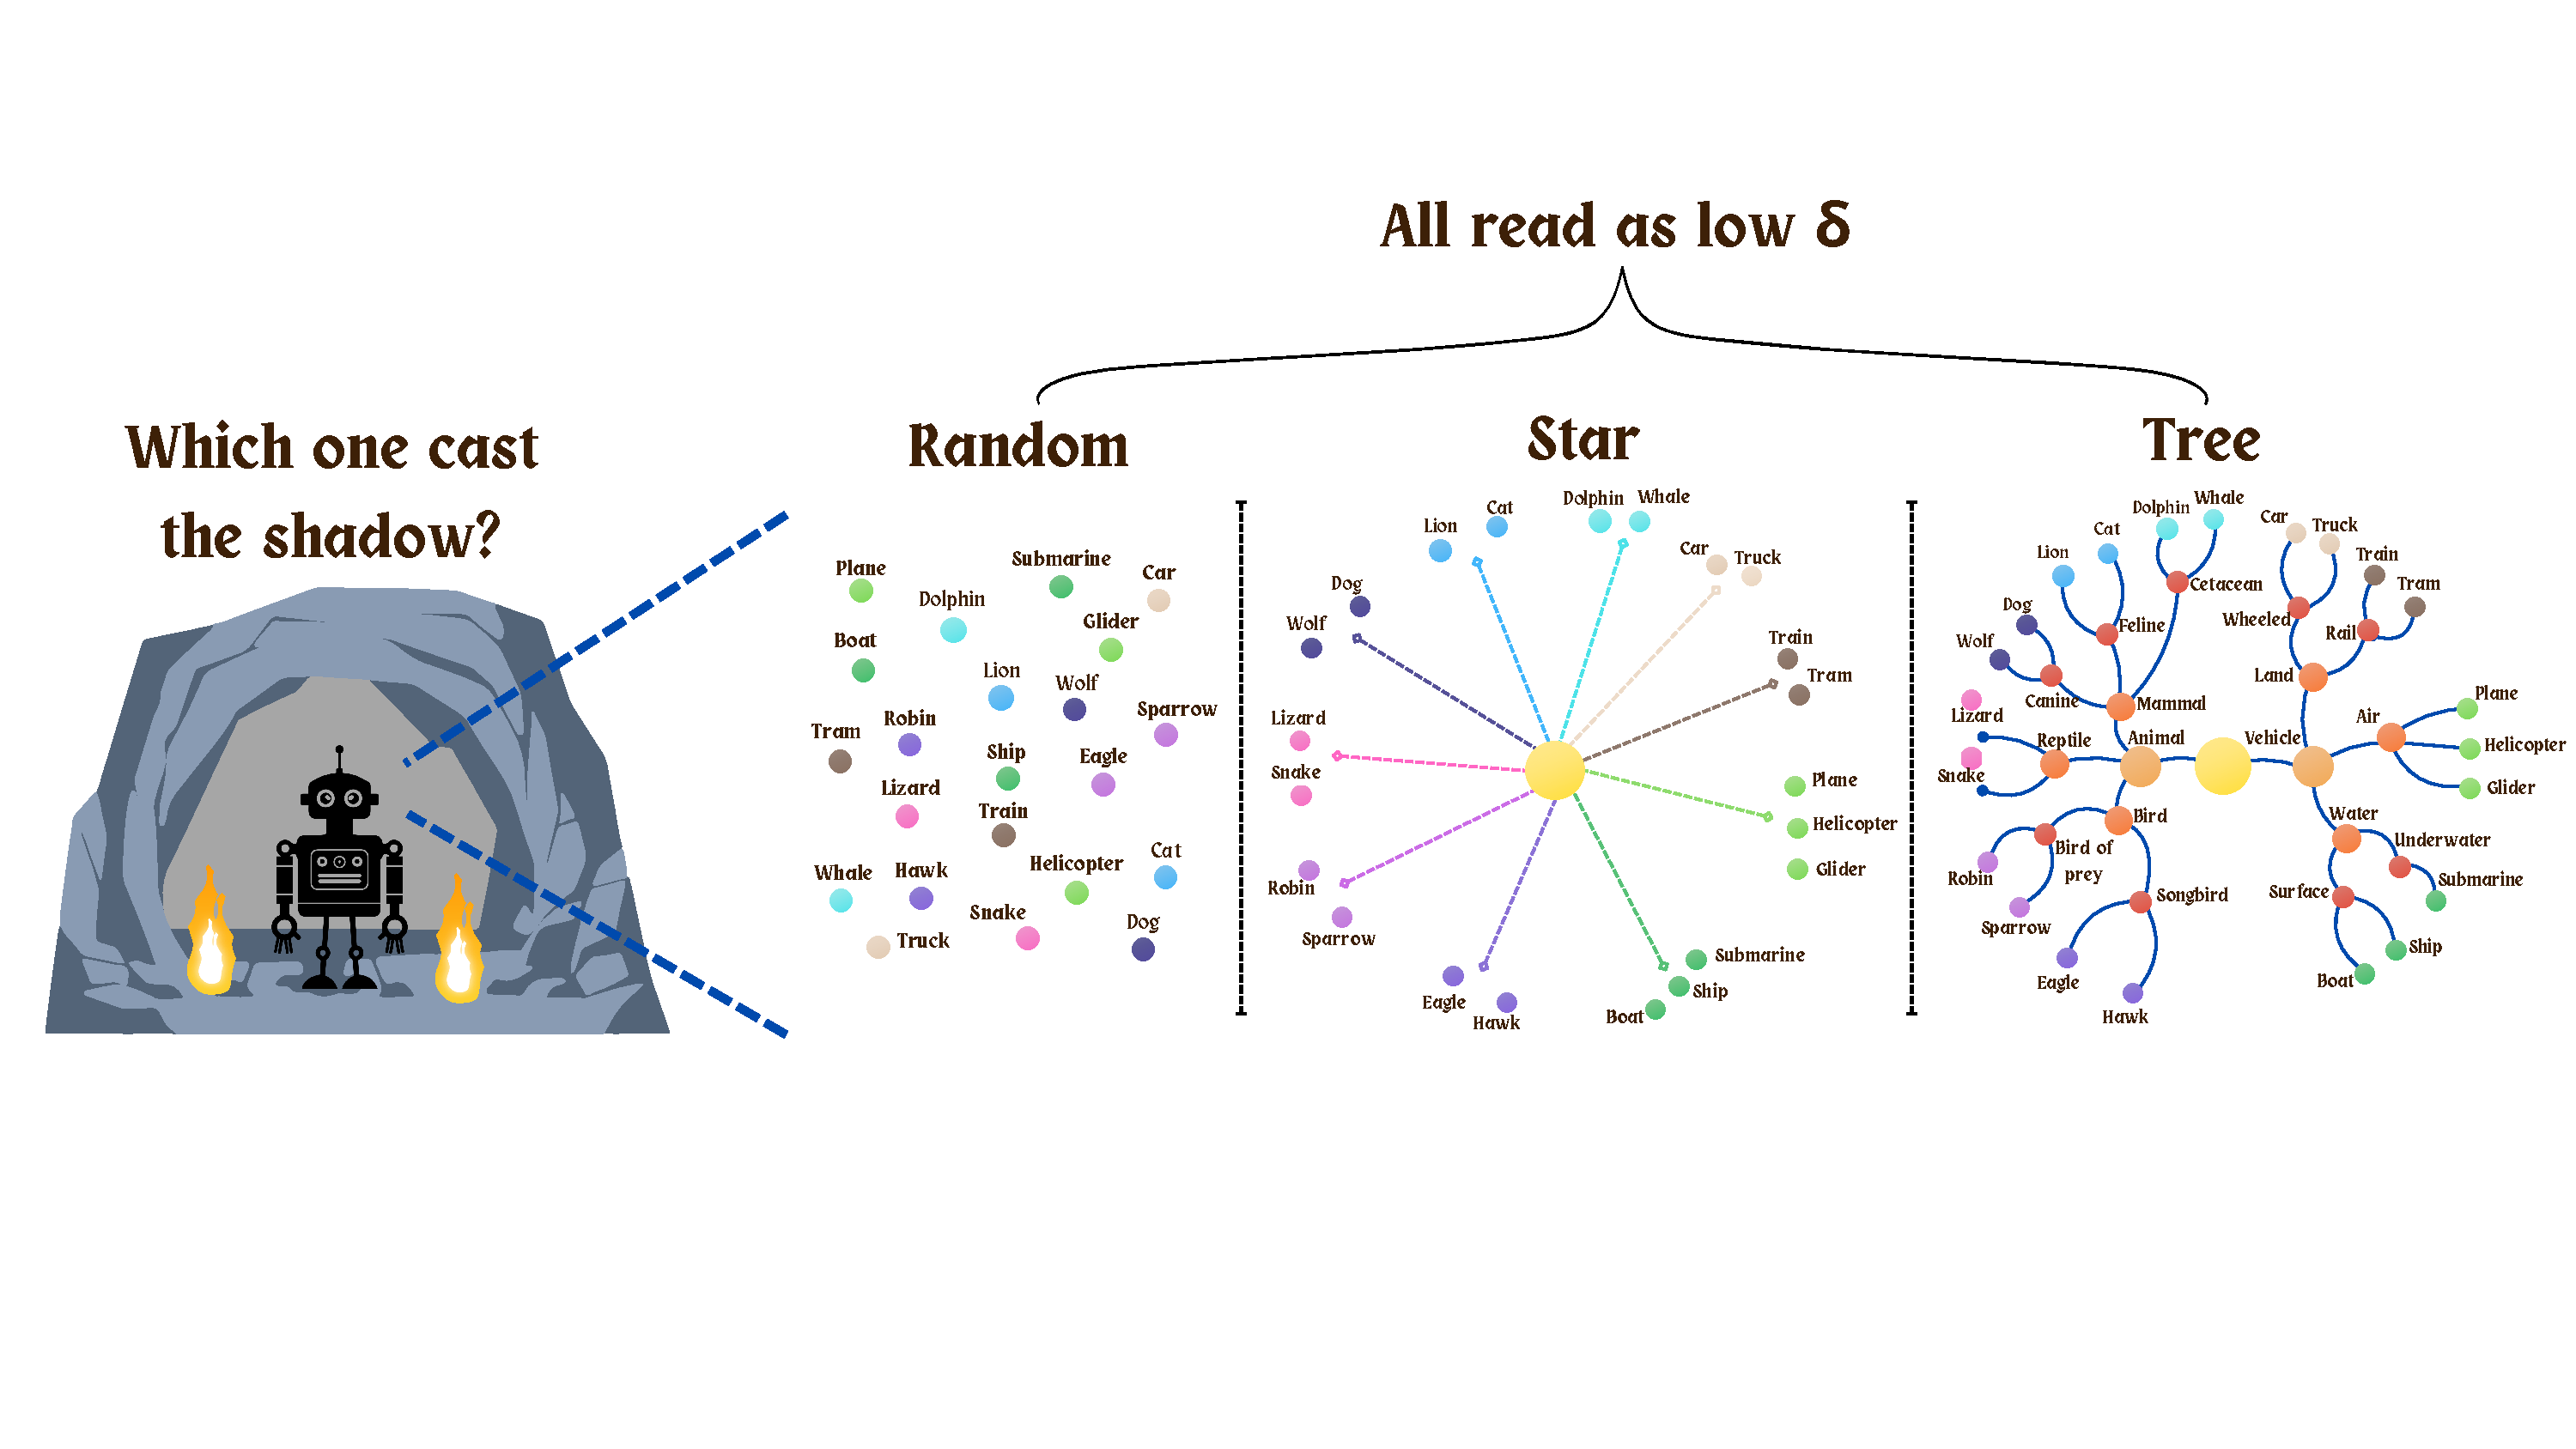
\includegraphics[width=\textwidth, trim=23 229 3 232]{figures/fig1_concept.pdf}}
{\fbox{\parbox[c][1.4in][c]{\dimexpr\textwidth-2\fboxsep-2\fboxrule\relax}{\centering \texttt{figures/fig1\_concept.pdf} (conceptual figure, drawn by the authors; same-size placeholder)}}}
\vspace{2pt}
\caption{\textbf{Plato's cave: a random cloud, a star and a tree cast the same shadow.} An observer who sees only shadows cannot tell which object cast them, and a raw $\delta$ is such a shadow: points with no structure, clusters around a center, and a nested hierarchy all read as low $\delta$. The instrument reads the objects instead of the shadow: the excess separates the random cloud from the other two, and the second test separates the star from the tree.}
\label{fig:concept}
\end{figure}

Why is the reading low? Gromov $\delta$ assigns zero to trees \citep{Gromov1987}, but its reference level depends on dimension, spectrum and statistic, so a raw value cannot be called low on its own. High-dimensional clouds concentrate toward equidistance \citep{beyer1999nearest, aggarwal2001surprising}, which is a degenerate star tree: we call this the \emph{dimension confound}, the geometric counterpart of the width confounder of \citet{groger2026aristotelian}. Anisotropic spectra lower the effective dimension and raise the reading: the \emph{spectrum confound}. And computing the supremum exactly takes more than cubic time \citep{fournier2015computing}, so it is taken over sampled quadruples, where it grows with the budget and does not converge: the \emph{statistic confound}.

We build the instrument that reads $\delta$ against the right reference. It calibrates the estimator on reference geometries, expresses every reading as an \emph{excess} over a null cloud matched in dimension and covariance spectrum, ranks that excess against matched replicates, and adds a \emph{second test} whose false-alarm rate and power are measured on real clouds. With it we ask of geometry what convergence work asks of similarity \citep{huh2024platonic, groger2026aristotelian}: what survives calibration, and is it shared? \citet{groger2026aristotelian} calibrate similarity across models; we calibrate geometry within a model, and comparing trees across models needs a calibration of its own.

\textbf{The answer has three parts.} (i) \emph{Where the premise is read,} on image features, the calibrated reading is indistinguishable from a random cloud of the same shape in most model--dataset cells and small elsewhere. The 4 values reported by \citet{Khrulkov_2020_CVPR} are reproduced and, calibrated, only MiniImageNet is genuine. CIFAR-10 and CUB-200 are indistinguishable from a random cloud, and CIFAR-100 falls below it only before correction ($p=0.030$). (ii) \emph{Within each model,} class centroids carry structure that a random cloud does not have, in 44 of 72 cells and 30 of 36 on datasets with 47 classes or more, but a star of clusters already produces it. The second test finds more in 4 of 12 ImageNet backbones: how each cluster is oriented relative to its superclass center, not a hierarchy among those centers. Rotating each cluster at random removes every verdict, whereas a hierarchy we plant ourselves, synthetic or trained into a model, survives. In the 9 of 12 backbones where a planted hierarchy is detected, none as strong is found; in the other 3 the test cannot see a planted hierarchy. A backbone trained in hyperbolic space shows the same structure as its Euclidean twin and stays nearly flat. (iii) \emph{Across models,} the trees agree on which classes group together well above chance, though less than two readings of the same model, and not on distances; the self-supervised models organize classes by direction rather than by distance, which a comparison by distance misses.

\textbf{Our contributions are:}
\begin{enumerate}[topsep=0pt,itemsep=1pt,leftmargin=*]
\item \textbf{The instrument.} A calibrated reading of $\delta$, compared with random clouds of the same shape, and a second test whose false-alarm rate and power are measured on real clouds.
\item \textbf{The census.} The premise calibrated where it is read, including a published reading reproduced; structure beyond a random cloud in most models; non-random orientation of clusters relative to their superclass centers in a few; no hierarchy among those centers where the test can see one; and a hyperbolic-trained backbone as the control for imposing the geometry.
\item \textbf{The map of trees.} Across models, the trees agree on which classes group together but not on distances, and the self-supervised models organize classes by direction, which a comparison by distance misses.
\item \textbf{Consequences for practice.} The rule that derives curvature from a raw $\delta$ assigns curvature to random clouds; we say what to measure before imposing curvature, and cosine collects most of the structure at no cost.
\end{enumerate}

\section{Related Work}
\label{sec:related}

Reading $\delta$ against a matched reference has precedent in network science, where the $\delta$ of real graphs is compared with that of random graphs of comparable size \citep{narayan2011curvature, kennedy2013hyperbolicity, adcock2013treelike}. We bring the idea to embedding clouds, where the reference must match dimension and spectrum. The curvature itself has been studied as a representation tradeoff \citep{sala2018representation} and as a mixed-curvature product to be learned \citep{gu2019learning}. In few-shot learning \citet{moreira2024hyperbolic} find that fixed-radius Euclidean prototypes match hyperbolic ones. The analyses of learned representations characterize Euclidean structure and do not test for tree-likeness: representation similarity, intrinsic dimension and neural collapse \citep{kornblith2019cka, ansuini2019intrinsic, pope2021intrinsic, papyan2020prevalence}. Closest to us is the work on representational convergence: the Platonic Representation Hypothesis \citep{huh2024platonic} argues that models converge toward shared representations, and its cross-modal convergence has been stress-tested at scale \citep{koepke2026cave}; \citet{groger2026aristotelian} show that permutation-calibrated similarity removes most of that convergence while local neighborhood structure survives, and \citet{park2024geometry} read concept hierarchy in language models from the orthogonality of concept directions. We are the geometric complement of this program: the same calibration applied within a model instead of across models.

\section{Methodology}
\label{sec:instrument}

\subsection{Background: Gromov $\delta$}
\label{sec:f-gromov}

Tree-likeness is measured on quadruples. Take any four points $w,x,y,z$ of a metric space with distance $d$. They can be paired in three ways, and each pairing has a sum of two distances:
\begin{equation}
d(w,x)+d(y,z),\qquad d(w,y)+d(x,z),\qquad d(w,z)+d(x,y).
\label{eq:pairings}
\end{equation}
Sort the three sums as $S_{\max}\ge S_{\mathrm{mid}}\ge S_{\min}$. In a tree the two largest sums are always equal, because the two pairings that cross the trunk traverse the same path, so the four-point defect $(S_{\max}-S_{\mathrm{mid}})/2$ is zero. The further a metric is from a tree, the larger the defect can become. A metric tree has $\delta=0$. Euclidean space has no bound at all: enlarging a square enlarges its defect in proportion. Hyperbolic space sits in between, with a bounded defect whose value for the hyperbolic plane is known, $\ln 2$ under this definition \citep{nica2016strong}.

\begin{defbox}
\begin{definition}[four-point defect]
\label{def:defect}
For a quadruple $(w,x,y,z)$ with the pairing sums of Eq.~\ref{eq:pairings} sorted as $S_{\max}\ge S_{\mathrm{mid}}\ge S_{\min}$, the four-point defect is $\delta(w,x,y,z)=\tfrac12\,(S_{\max}-S_{\mathrm{mid}})$, and the Gromov $\delta$ of a metric space is the supremum of the defect over its quadruples \citep{Gromov1987}.
\end{definition}
\end{defbox}

\subsection{Estimation and normalization}
\label{sec:f-estimation}

Three steps turn $\delta$ into a number that can be compared across models. First, a thousand centroids have far more quadruples than can be enumerated, and exact computation takes more than cubic time \citep{fournier2015computing}. The defect is therefore computed on half a million random quadruples. Second, the largest defect in that sample is a poor estimate of the supremum: it belongs to a single extreme quadruple and keeps growing as more quadruples are drawn. We therefore read the 99.9th percentile of the sampled defects, $\hat\delta_{99.9}$, the value that 99.9 per cent of them fall below. It keeps the tail of the defects, as the supremum does, but it is set by hundreds of quadruples rather than by one. It also does not move with the sample size: across quadruple budgets the ImageNet reading drifts by less than half its own spread (Figure~\ref{fig:budget}). Third, the defect grows with the size of the point set, so we divide by the diameter, the largest pairwise distance:
\begin{equation}
\delta_{\text{norm}}=\frac{\hat\delta_{99.9}}{\mathrm{diam}}.
\label{eq:deltanorm}
\end{equation}
On this scale a tree reads zero, and a hyperbolic region of radius four or more reads below a sphere (Table~\ref{tab:q10-calibration}).

\begin{defbox}
\begin{definition}[reading]
\label{def:reading}
$\delta_{\text{norm}}$ of Eq.~\ref{eq:deltanorm}, with $\hat\delta_{99.9}$ computed over half a million sampled quadruples per seed and averaged over 10 seeds, is the statistic used throughout; we call it the reading.
\end{definition}
\end{defbox}

\begin{propbox}
\begin{proposition}[range bound and dimension confound]
\label{prop:bound}
Let $d_{\min}$ and $d_{\max}$ be the smallest and the largest pairwise distance of a finite metric space. (a) For any quadruple the four-point defect is at most $d_{\max}-d_{\min}$, hence $\delta_{\text{norm}}\le 1-d_{\min}/d_{\max}$. (b) For an iid Gaussian cloud of $n$ points in dimension $d$, with $n$ fixed, $d_{\min}/d_{\max}\to1$ as $d$ grows \citep{beyer1999nearest, aggarwal2001surprising}, so $\delta_{\text{norm}}\to0$ without any structure.
\end{proposition}
\end{propbox}

\paragraph{A raw value cannot be called low on its own.} Proposition~\ref{prop:bound} makes the dimension confound precise; the calibration on reference geometries shows the spectrum and statistic confounds (Table~\ref{tab:q10-calibration}).

\subsection{Spectrum-matched null, excess and genuineness}
\label{sec:f-null}

\begin{defbox}
\begin{definition}[Haar null]
\label{def:null}
A null replicate is a cloud with the real shape and no structure. Let $X=U\Sigma V^{\top}$ be the singular value decomposition of the centered cloud; the replicate is $X'=Q\Sigma V^{\top}$ with $Q$ the orthogonal factor of a column-centered Gaussian matrix, orthogonal to the all-ones vector and Haar-distributed on the centered subspace, so $X'$ has exactly the centered singular values of $X$ and structureless coefficients.
\end{definition}
\end{defbox}

\paragraph{Of the two constructions, one reproduces the shape exactly.} Of the two compared, Gaussian coefficients reproduce the spectrum only on average and inflate the excess of low-rank clouds. The centered Haar construction reproduces the centered spectrum exactly, so it is the null used throughout. The uncentered and the Gaussian readings are reported beside it (Table~\ref{tab:q1-census-b}).

\begin{defbox}
\begin{definition}[excess]
\label{def:excess}
With $K$ null replicates $X'_1,\dots,X'_K$ of Definition~\ref{def:null}, the excess of a cell is
\begin{equation}
e(X)=\delta_{\text{norm}}(X)-\frac{1}{K}\sum_{k=1}^{K}\delta_{\text{norm}}(X'_k).
\label{eq:excess}
\end{equation}
\end{definition}
\end{defbox}

\paragraph{Size and evidence.} The excess is a size, the gap between a reading and its random cloud in Figure~\ref{fig:instrument}a. The evidence is the rank of the reading among its replicates and the left-tail $p$ that the rank gives,
\begin{equation}
r=\#\{k:\ \delta_{\text{norm}}(X'_k)>\delta_{\text{norm}}(X)\},\qquad p=\frac{1+K-r}{K+1},\qquad K=200.
\label{eq:rank}
\end{equation}

\begin{defbox}
\begin{definition}[genuine]
\label{def:genuine}
Order the $m$ left-tail $p$-values of a census as $p_{(1)}\le\dots\le p_{(m)}$. A model--dataset cell is genuine when its $p$ is at or below the Benjamini--Hochberg threshold \citep{benjamini1995controlling} at level five per cent,
\begin{equation}
p\ \le\ p_{(i^{*})},\qquad i^{*}=\max\{i:\ p_{(i)}\le 0.05\, i/m\},
\label{eq:bh}
\end{equation}
and the word is used in this sense only.
\end{definition}
\end{defbox}


\paragraph{What a genuine excess means.} A negative genuine excess, more than chance would give, certifies structure beyond the second moments; clustering is its most plausible reading, supported by the superclass recovery of Section~\ref{sec:content}. Two cells of the same dataset can have the same reading, $0.082$, ViT-B on CIFAR-100 images and DINO-B on its centroids, and only the second is genuine.


\begin{figure}[t]
\centering

\includegraphics[width=\linewidth]{figures/fig_instrument_final.pdf}
\caption{\textbf{The instrument in one figure.} (a) Raw reading, a random ball of the same dimension, and a random cloud of the same shape; the ball-to-cloud gap is the spectrum's share and the cloud-to-model gap is the excess. (b) Their difference, the excess, filled when genuine. (c) The hierarchy test on the real cloud, with its orientations randomized, and on a planted hierarchy randomized the same way. (d) The test's power for the planted hierarchy, intact and randomized; whiskers: 95 per cent intervals over 50 runs per backbone, 200 for the DINOv2 family. % expR75_census_centered_haar.csv, expR74_decoupling_summary.csv, expR81_deep_per_backbone_summary.csv
}

\label{fig:instrument}
\end{figure}

\subsection{Hierarchy test}
\label{sec:f-depthtest}

\paragraph{Why a second test.} A genuine excess can come from clusters alone, so a second test, which we call the hierarchy test, asks whether the clusters are themselves arranged hierarchically. It needs three constructions.

\begin{defbox}
\begin{definition}[hub null and hub excess]
\label{def:hubnull}
Given a grouping of classes into superclasses, assigning each centroid $x_i$ to a cluster $k(i)$ with hub $h_{k(i)}$, the cluster mean, write $x_i=h_{k(i)}+o_i$. The hub null keeps every offset $o_i$ and replaces the hubs by a Haar resample with their spectrum, $x'_i=h'_{k(i)}+o_i$, and the excess of Eq.~\ref{eq:excess} against this null, $e_{\mathrm{hub}}$, measures structure above the clusters of the grouping only.
\end{definition}
\end{defbox}

\begin{defbox}
\begin{definition}[matched star]
\label{def:star}
The matched star of a cloud keeps the real clusters, each as a Haar sample with the cluster's own covariance, and places their hubs as Gaussian draws at the real hub radius: the clustering of the real cloud with no hierarchy above it. Its spectrum-matched-hub variant draws the hubs as a Haar resample of the real hubs.
\end{definition}
\end{defbox}

\begin{defbox}
\begin{definition}[rotating each cluster]
\label{def:decoupling}
This control keeps the hubs of the grouping and rotates each cluster's offsets by an independent Haar rotation. A verdict that survives the rotation is carried by the arrangement of the hubs; one that does not is carried by the orientation of the clusters relative to their hubs, which we call alignment.
\end{definition}
\end{defbox}

\paragraph{The hierarchy test compares the real cloud with its matched star.} With $e_{\mathrm{hub}}$ read on the real cloud and on its matched star, the depth statistic and its standardized form are
\begin{equation}
\mathrm{depth}=e_{\mathrm{hub}}(X)-e_{\mathrm{hub}}(X_{\mathrm{star}}),\qquad z=\mathrm{depth}\,/\,\mathrm{s.d.},
\label{eq:depth}
\end{equation}
where the spread is taken over star seeds and null replicates, and a cloud is certified against its matched star when $z\le-2$. The power of the test is the fraction of planted hierarchies it detects, and its false-alarm rate is the fraction of flat controls that fire. Both are measured in Section~\ref{sec:f-depth}.


\subsection{Comparing trees across models}
\label{sec:f-treemap}

\paragraph{Trees are compared under a configuration chosen before the comparison.} Two hierarchies are compared by the adjusted Rand index between their cut partitions and by the correlation of their cophenetic distances. They are also compared by their agreement on which pair of a random class triplet merges first. The configuration of metric and linkage is selected per dataset by a criterion fixed without reference to the agreements. It is the highest cophenetic fidelity among configurations whose reference cuts are non-degenerate for every model. Local agreement is read with the permutation calibration of \citet{groger2026aristotelian} on mutual-kNN agreement and centroid CKA.

\subsection{Projection and tasks}
\label{sec:f-projection}

\paragraph{Three metrics are compared on the intact representation.} A parameter-free map centers the features, scales the 95th-percentile norm to radius $1/\sqrt2$ and preserves directions. Euclidean, cosine and Poincar\'{e} metrics are then scored by nearest-centroid classification and 5-way 5-shot episodes on every cell of the task grid. % exp1, exp2

\section{Experimental Setup}
\label{sec:f-setup}

\paragraph{The census, the reading of every model--dataset cell, has 12 backbones, 6 class sets and 15 text models.} The vision backbones are 4 supervised ViTs \citep{dosovitskiy2021an} trained on ImageNet-21k \citep{imagenet}, DINO-B \citep{dinov1}, 4 DINOv2 sizes \citep{dinov2}, CLIP-B, CLIP-L \citep{CLIP} and SigLIP-B \citep{siglip}. The class sets are ImageNet (1000 classes) and CIFAR-100 \citep[100 classes;][]{cifar10}, which carry a real hierarchy; DTD \citep[47 classes;][]{dtd} and CIFAR-10 (10 classes); and the flat FashionMNIST \citep[FMNIST, 10 classes;][]{fashion} and MNIST \citep[10 classes;][]{mnist}. The text models read the thousand ImageNet class names: 4 GPT-2 sizes \citep{gpt2}, 3 Pythia sizes \citep{pythia}, OLMo-1B \citep{olmo} and 7 sentence embedders (Table~\ref{tab:q14-panel}).

\paragraph{Four controls test the alternatives.} Two self-supervised ResNets \citep{resnet,zbontar2021barlow,grill2020bootstrap} read the vision census. DeiT-B \citep{deit} and the augreg ViT-B \citep{augreg}, trained on ImageNet-1k leaf labels, test whether a hierarchical label set explains the alignment. MERU and its Euclidean CLIP twin \citep{desai2023meru} test whether training in hyperbolic space creates hierarchy. The census ViT-B, fine-tuned with and without a hierarchical objective, is the trained control.

\paragraph{The premise is read on images and hierarchy on centroids.} The sample-level reading uses about a thousand stratified training images per cell on CIFAR-100 and DTD. Class centroids average a hundred cached training images per class on ImageNet and the full cached split elsewhere. Text models are read one prompt at a time, since batching alters GPT-2's hidden states, each with its own pooling (Table~\ref{tab:q14-panel}).

\paragraph{Calibration budget and groupings.} Each cell is read against 200 Haar replicates, with half a million sampled quadruples per seed and 10 seeds. With 10 classes there are only 210 quadruples, so $\hat\delta_{99.9}$ coincides with the supremum there. Benjamini--Hochberg runs over the vision census and, separately, over the text census. The grouping into superclasses is the WordNet \citep{wordnet} cut into 30 superclasses on ImageNet and the 20 coarse labels on CIFAR-100. A balanced grouping is the control, with 10 star seeds.

\section{Results}
\label{sec:form}

\subsection{The premise at the sample level}
\label{sec:f-sample}


\paragraph{The premise does not survive calibration where it is read.} On per-image features, where the premise is read, the calibrated reading is not genuine in 14 of 24 cells, that is, no more than chance would give. The excess is conservative: the null keeps the spectrum, so a hierarchy carried by the spectrum alone would not show. What fails is the evidence the premise cites, not the possibility of a hierarchy. Where it is genuine, the excess removes at most two fifths of the null reading. Figure~\ref{fig:premise}a and Table~\ref{tab:q3-sample} give the 24 cells. % expR62_samplelevel_record.csv

\paragraph{A published reading is reproduced and calibrated.} The estimator of \citet{Khrulkov_2020_CVPR}, run on our extraction, reproduces the raw $\delta_{\text{rel}}$ they report for ResNet-34 within 0.03. Calibrated, only MiniImageNet \citep{miniimagenet} is genuine. CIFAR-10 and CUB-200 \citep{cub} are indistinguishable from a random cloud, and CIFAR-100 falls below it only before correction ($p=0.030$). Under their own statistic, the supremum, CIFAR-10 and CUB-200 stay indistinguishable from a random cloud and MiniImageNet stays below it. The verdict for CIFAR-100 changes from trial to trial, as the statistic confound predicts. Figure~\ref{fig:premise}b and Table~\ref{tab:khrulkov} give the 4 datasets. % expR78_khrulkov_replication_summary.csv, expR85_khrulkov_sup_summary.csv

\begin{figure}[t]
\centering

\includegraphics[width=\linewidth]{figures/fig_premise_final.pdf}
\caption{\textbf{The premise where it is read.} (a) Excess of the reading on per-image features; filled: genuine, 10 of 24 cells. (b) The values reported by \citet{Khrulkov_2020_CVPR}, our reproduction with their estimator, and the random cloud of the same shape, all on their statistic: a dot inside the band is what chance gives. On their statistic CIFAR-10 and CUB-200 fall inside the band, MiniImageNet below it, and CIFAR-100 at its edge, its verdict changing from trial to trial (median rank 196/200); on our reading only MiniImageNet is genuine after correction, and CIFAR-100 falls below at $p=0.030$ before it (Section~\ref{sec:f-sample}). % expR62_samplelevel_record.csv, expR78_khrulkov_replication_summary.csv, expR85_khrulkov_sup.csv
}
\label{fig:premise}
\end{figure}

\subsection{Structure beyond the second moments at the class level}
\label{sec:f-class}


\paragraph{Most cells show structure beyond the second moments.} It is genuine, beyond a random cloud of the same shape, in 44 of 72 cells and 30 of 36 on the 3 datasets with 47 classes or more. On ImageNet and CIFAR-100 the count is 18 of 24. Figure~\ref{fig:excess} and Table~\ref{tab:census} give the census. % expR52_census_haar_p999_200.csv

\paragraph{The count survives resampling.} Folding image resampling and estimator seeds into the null spread, or repeating the census on resamples, keeps most of it. Table~\ref{tab:q8-robust-b} gives the bootstrap. % expR66_joint_sensitivity_summary.csv

\paragraph{A star of clusters already passes the census.} A synthetic star with no hierarchy scores an excess as deep as any real cell, so a negative excess says structure beyond the second moments, not a hierarchy. Table~\ref{tab:q10-calibration-b} gives the star's excess. % expR42_star_calibration.csv

\begin{figure}[t]
\centering

\includegraphics[width=\linewidth]{figures/fig_excess_final.pdf}
\caption{\textbf{Most cells show structure beyond the second moments.} (a) Excess of the reading over its matched null per dataset and backbone, filled when genuine; band: two null standard deviations. (b) The same reading for the 15 text models on the ImageNet class names; filled: genuine. % expR52_census_haar_p999_200.csv, expR53_text_haar_p999_200.csv
}
\label{fig:excess}
\end{figure}

\subsection{Hierarchy above the labelled clusters}
\label{sec:f-depth}

\paragraph{The hierarchy test certifies that how clusters are oriented relative to their hubs is not random in 4 of 12 backbones: ViT-S, ViT-B, ViT-L and DINOv2-L.} The test compares each cloud with its matched star, the same clusters with no hierarchy above them. It was run on the 12 ImageNet centroid clouds under both stars, with the WordNet grouping into superclasses and its centers as hubs. Figure~\ref{fig:instrument}c shows the $z$ per backbone and Tables~\ref{tab:q4-depth} and \ref{tab:q4-depth-ap} give both stars. % expR56_depth_variants.csv, expR69_depth_haarhubs_summary.csv

\paragraph{What it certifies is alignment, how each cluster is oriented.} Once each cluster is rotated at random, the control of Definition~\ref{def:decoupling}, none of the 4 backbones fires. ViT-L then reads $-1.61$, within the $-1.61$ to $-1.76$ of the flat control: without its orientations the real cloud reads like a flat one. The alignment is relational: 0 of 60 runs fire with random hubs and 0 of 4 with random orientations, so it needs both. Removing the radial component of every offset leaves it in all 4 certified backbones, $z$ from $-2.08$ to $-3.99$ under both stars; feature norms are not its source (Table~\ref{tab:q4-depth-e}). Under full L2 normalization, which also moves the hubs, it survives in ViT-B and ViT-L only. Its geometric form is not resolved here. % expR74_decoupling_summary.csv, expR79_synthetic_deep_poincare.csv, expR69_depth_haarhubs_summary.csv, expR64b_wn30.csv, expR82_radial_control.csv, expR80_implanted_alignment.csv

\paragraph{What the test can see.} The noise level of a cloud is its within-cluster spread relative to the distance between its hubs. Given a planted two-level tree at this noise level, the test misses it; given a three-level hierarchy with ViT-L's spectrum and noise, it detects it in 4 of 5 seeds. That detection survives orientation randomization, whereas none of the 4 real verdicts does. The same hierarchy was then built at each backbone's own spectrum and ratio. With clusters rotated the control detects it in 9 of 12 backbones (power 0.83--1.00) over 50 to 200 runs per backbone, and not in the other 3 (power 0.01--0.60). ViT-S and DINOv2-B sit closest to the threshold, with 95 per cent intervals reaching 0.79 and 0.78. The 3 that cannot see a planted hierarchy, ViT-T, DINO-B and DINOv2-S, sit at noise levels 1.5 to 3.0, inside the 1.3 to 3.9 spanned by the 9 covered backbones. The power follows the backbone, not its noise level or family. % expR64b_wn30_summary.csv, expR79_synthetic_deep_poincare.csv, expR81_deep_per_backbone.csv, expR81_deep_per_backbone_summary.csv

\paragraph{A trained hierarchy survives, and the test leans toward firing with clusters rotated.} ViT-B fine-tuned with a hierarchical cross-entropy keeps firing with its clusters rotated in 20 of 20 runs over 2 seeds, mean $z$ $-2.51$, on the WordNet grouping. The leaf-only fine-tune fires in 6 of 20, mean $z$ $-1.37$, and the frozen checkpoint in none. Fine-tuning itself adds some signal with clusters rotated and the hierarchical objective adds more, so the trained control separates the objectives by degree. A flat control with the same spectrum and ratio as the deep one fires in 0 of 5 intact runs and in 8 of 50 runs with clusters rotated. The test is therefore biased toward firing, so the failure of the 4 real backbones to fire once rotated is conservative evidence. The synthetic hierarchy at $z$ $-4.19$ to $-4.82$ stands well clear of that bias. On the balanced grouping the matched flat control fires in 0 of 50 runs with clusters rotated. Tables~\ref{tab:q5-power-d} and \ref{tab:q4-depth-d} give the runs. % expR77_positive_control.csv, expR77_positive_control_verdict.json, expR79_synthetic_deep_poincare.csv, expR83_flat_balanced_summary.csv

\paragraph{No hub hierarchy is found where the test has power.} In those 9 backbones, none as strong as the planted one is found. Rotating each cluster separates structure among the hubs of the grouping from structure carried by cluster orientations. A hierarchy below the grouping expressed in how clusters open would be removed with the orientations and counted as alignment. No hub hierarchy therefore means no hierarchy among the grouping's hubs. Figures~\ref{fig:implant} and \ref{fig:power} give the detection rates and the power. % expR81_deep_per_backbone_summary.csv, final_wordnet_levels.json, expR64b_wn30.csv

\paragraph{The certified set depends on the grouping.} Rerun under a balanced grouping, ViT-T joins the certified set and ViT-S and DINOv2-L leave it; other WordNet cuts change the set again (Table~\ref{tab:q4-depth}). % expR56_depth_variants.csv, expR64b_wn30bal_summary.csv

\paragraph{Leaf labels can produce the alignment but do not guarantee it.} Read like the census models, the augreg ViT-B trained on ImageNet-1k leaf labels is certified, and DeiT-B, trained on the same labels with another recipe, is not (Table~\ref{tab:q4-depth-b}). % expR70_inet1k_supervised.csv

\paragraph{Training in hyperbolic space leaves the clustering unchanged.} Read with the census and the hierarchy test, MERU shows the same clustering as its Euclidean twin. No hub structure is detected, although the test's power at MERU's spectrum was not measured. Its embeddings also stay nearly flat: 95 per cent lie within 0.29 of the curvature scale (Table~\ref{tab:q4-depth-c}). % expR63_meru_record.csv, expR71_meru_radii.csv

\subsection{Whose tree}
\label{sec:content}

\begin{figure}[t]
\centering

\includegraphics[width=\linewidth]{figures/fig_treemap_final.pdf}
\caption{\textbf{The island is the cut; tree topology is shared well above chance, though short of the within-model ceiling; the self-supervised structure is angular.} (a) Mean agreement of each model's tree with the other 11, naive (hollow) and corrected (filled). (b) Triplet agreement under the corrected comparison against the within-model ceiling (band). (c) Sibling-triplet agreement under cosine and Euclidean distance. % exp23_treemap_controls.npz, expR58_treemap_cutfree.csv, expR84_tree_ceiling.csv, exp10_local_vs_global.csv
}
\label{fig:treemap}
\end{figure}

\paragraph{The naive map manufactures an island.} Compared with Euclidean distances and average linkage, the DINOv2 models agree with none of the others, an island in the map of models. They agree with the 7 supervised and contrastive models far less than those 7 agree among themselves (DINO-B is not part of the island). The cause is chaining: DINOv2's Euclidean dendrograms put almost every class in one cluster, forcing the index to zero (Figure~\ref{fig:treemap}a). % exp23_treemap_controls.npz, exp23_config_diagnostics.json

\paragraph{Controlled, the trees share their topology, not their metric.} Across models, triplet agreement reaches 0.77, against 0.90 for two resamples of the same model. Chance gives 0.33. The cophenetic and cut agreements reach about half their within-model ceiling (Table~\ref{tab:q6-treemap-b} and Figure~\ref{fig:treemap}b). Calibrated local agreement across models survives, as \citet{groger2026aristotelian} find for similarity (Table~\ref{tab:q13-local}). % exp23_treemap_controls.npz, expR58_treemap_cutfree_summary.csv, expR84_tree_ceiling_summary.csv, exp21b_local_global_K200.csv

\paragraph{The self-supervised tree is angular.} Sibling triplets were resolved under cosine and under Euclidean distance: DINOv2 resolves them far better under cosine, so its semantics concentrate in the angular component and its Euclidean dendrograms chain. Repeated on cosine geometry, the census agrees with the Euclidean one in most cells, and DINOv2 on ImageNet is genuine, more than chance would give, under both. Figure~\ref{fig:treemap}c shows the triplets and Table~\ref{tab:q1-census-c} gives the cosine census. % exp10_local_vs_global.csv, expR57_census_cosine_haar_p999_200.csv

\paragraph{Agreement with WordNet follows supervision.} The correlation between inter-centroid and WordNet distances is highest for the contrastive VLMs ($+0.57$ to $+0.59$), then the supervised ViTs ($+0.49$ to $+0.53$), and lowest for DINOv2 ($+0.18$ to $+0.22$). On DBpedia Classes \citep{dbpedia} and on HierarCaps \citep{alper2024hierarcaps}, two hierarchies independent of WordNet, the text encoders read a genuine excess and resolve sibling triplets far above chance. Tables~\ref{tab:q7-wordnet}, \ref{tab:q7-wordnet-c} and \ref{tab:q7-wordnet-d} give the three readings. % exp3_alignment.csv, expR61_dbpedia_record.csv, exp27_dbpedia_treemap.json, exp16_hierarcaps.csv

\paragraph{Text depends on recipe and scale.} 7 of 15 text models are genuine under the reading (Figure~\ref{fig:excess}b). GPT-2 L and XL are genuine under every reading while S and M change with it. Pythia is genuine at every size. The sentence embedders are not genuine on class names (Table~\ref{tab:q2-text}). % expR53_text_haar_p999_200.csv, expR49_template_nulls_bs1.csv, expR47_extraction_variance.csv, expR61_dbpedia_record.csv

\section{Implications for Hyperbolic Representation Learning}
\label{sec:practice}

\paragraph{The raw reading cannot select a curvature.} \citet{Khrulkov_2020_CVPR} set the curvature of the Poincar\'{e} ball from the relative hyperbolicity, $c=(0.144/\delta_{\text{rel}})^{2}$ with $\delta_{\text{rel}}=2\delta/\mathrm{diam}$. Applied, with the supremum it was calibrated for, to structureless Gaussian clouds, it assigns curvatures from 0.48 to 2.5. The raw and calibrated readings predict the gain of a non-Euclidean metric equally well, and the hierarchy verdict predicts none (Table~\ref{tab:q9-corollary-d}). Calibration tells what a low $\delta$ means, not which metric to use. The Poincar\'{e} metric adds $+0.9$ to $+1.3$ pp over cosine for the contrastive VLMs on prototype tasks and nothing consistent elsewhere (Table~\ref{tab:q9-corollary}). We test zero-cost metrics only; whether hyperbolic training helps for other reasons is outside this study. % exp1_delta_controls.csv, expR68_corollary_excess.csv, exp24_val_metric_selection.csv, exp2b_normalized_stack.csv, exp2_metric_controls.csv


\section{Conclusion and Limitations}
\label{sec:discussion}

\paragraph{Conclusion.} Read correctly, foundation models organize classes into clusters that they partly share and show no hierarchy among the superclasses where the test can see one. Their raw tree-likeness is not evidence for hyperbolic geometry.

\paragraph{Limitations.} (i)~The spectrum null conditions on the second moments, to which a hierarchy contributes, so a low excess over it does not exclude hierarchy carried by the spectrum. (ii)~The verdict of no hub hierarchy holds only in the 9 of 12 backbones where the control with clusters rotated detects a planted hierarchy. (iii)~The text census depends on the probe: template and batching move the reading, so marginal verdicts are fragile. (iv)~The analysis rests on many choices, groupings, stars and null variants among them; a pre-specified analysis is future work. (v)~The census is class-centroid geometry on 6 datasets, and the sample-level reading covers 2 datasets, one budget and one setting. (vi)~The reading divides by the diameter, so heavier tails would lower $\delta_{\text{norm}}$ without any clustering; the cosine census mitigates this. (vii)~The hierarchy test is Euclidean and may be conservative for the angular DINOv2 tree; the objective--geometry link is correlational. % expR47_extraction_variance.csv, expR49_template_nulls_bs1.csv, expR81_deep_per_backbone_summary.csv

\subsubsection*{Reproducibility Statement}
The supplementary material contains the scripts that produce every result in the paper, with fixed seeds, and a README that maps each result to its script; its \texttt{tool/} directory ships the instrument as one script that reproduces any cell of Table~\ref{tab:census} from its centroid matrix.

\subsubsection*{Ethics Statement}
This work analyzes publicly released models and standard public datasets, involves no human subjects and no personal data, and proposes an analysis methodology. We do not foresee ethical risks beyond those already associated with the underlying models and datasets.

\subsubsection*{AI Use Statement}
We used generative AI tools to assist with writing and editing, retrieving references, and implementing and running the experimental code, and to give feedback on drafts and on the methodology. We reviewed and verified all AI-assisted work, including every number, figure and reference, and take full responsibility for the content of this paper.

\FloatBarrier
\bibliographystyle{iclr2027_conference}
\bibliography{references}

\clearpage
\appendix
\raggedbottom
\section{Proofs}\label{app:proofs}

\textbf{Proposition~\ref{prop:bound}} (range bound and dimension confound).
\emph{Let $d_{\min}$ and $d_{\max}$ be the smallest and the largest pairwise distance of a finite metric space.
(a) For any quadruple, the four-point defect is at most $d_{\max}-d_{\min}$; hence $\delta_{\text{norm}} \le 1 - d_{\min}/d_{\max}$.
(b) For an iid Gaussian cloud of $n$ points in dimension $d$, with $n$ fixed, $d_{\min}/d_{\max}\to 1$ as $d$ grows, so $\delta_{\text{norm}}\to 0$ without any structure.}

\paragraph{Intuition.} The defect is half the difference between two sums of distances. If all distances are nearly equal, every sum is nearly equal, and the difference cannot be large. Part (a) makes this exact; part (b) shows that a random cloud in high dimension has nearly equal distances.

\paragraph{Proof of (a).} Take any four points and their three pairing sums (Eq.~\ref{eq:pairings}). Each sum adds two distances, and every distance lies between $d_{\min}$ and $d_{\max}$, so every sum lies between $2d_{\min}$ and $2d_{\max}$:
\begin{equation}
2d_{\min} \;\le\; S_{\min} \;\le\; S_{\mathrm{mid}} \;\le\; S_{\max} \;\le\; 2d_{\max}.
\end{equation}
The defect is therefore bounded by the width of that interval:
\begin{equation}
\tfrac12\bigl(S_{\max}-S_{\mathrm{mid}}\bigr) \;\le\; \tfrac12\bigl(2d_{\max}-2d_{\min}\bigr) \;=\; d_{\max}-d_{\min}.
\end{equation}
The bound holds for every quadruple, so it holds for their supremum $\delta$ and for any percentile of the sampled defects, which never exceeds the supremum. The diameter of the set is $d_{\max}$; dividing by it gives
\begin{equation}
\delta_{\text{norm}} \;\le\; \frac{d_{\max}-d_{\min}}{d_{\max}} \;=\; 1-\frac{d_{\min}}{d_{\max}}. \qquad\square
\end{equation}

\paragraph{Proof of (b).} Let $x_1,\dots,x_n\in\mathbb{R}^d$ have iid standard Gaussian coordinates. For one pair $i\neq j$, the squared distance is a sum of $d$ independent terms:
\begin{equation}
\|x_i-x_j\|^2 \;=\; \sum_{k=1}^{d}\bigl(x_{ik}-x_{jk}\bigr)^2 .
\end{equation}
Each term is the square of a Gaussian of variance 2, so it has mean 2. By the law of large numbers, the average of the $d$ terms tends to its mean:
\begin{equation}
\frac{\|x_i-x_j\|^2}{2d} \;\longrightarrow\; 1 \qquad \text{almost surely, as } d\to\infty .
\end{equation}
With $n$ fixed there are finitely many pairs, $n(n-1)/2$, so the convergence holds for all of them at once, and in particular for the smallest and the largest distance:
\begin{equation}
\frac{d_{\min}}{\sqrt{2d}} \to 1, \qquad \frac{d_{\max}}{\sqrt{2d}} \to 1, \qquad\text{hence}\qquad \frac{d_{\min}}{d_{\max}} \to 1 .
\end{equation}
Part (a) then gives $\delta_{\text{norm}} \le 1-d_{\min}/d_{\max} \to 0$. The relative contrast between the farthest and the nearest pair vanishes at rate $d^{-1/2}$ \citep{beyer1999nearest, aggarwal2001surprising}: this is the dimension confound, with no structure in the cloud. $\square$

\renewcommand{\topfraction}{0.95}\renewcommand{\bottomfraction}{0.95}\renewcommand{\textfraction}{0.03}\renewcommand{\floatpagefraction}{0.85}\setcounter{topnumber}{4}\setcounter{bottomnumber}{4}\setcounter{totalnumber}{6}\renewcommand{\arraystretch}{0.92}
% final version: the tables float ([tbp], one float per panel) within their subsection (a \FloatBarrier closes each one)
\section{Implementation}
\label{app:panel}
\paragraph{What this table answers.} Every model named anywhere in the paper appears here once, with its size and its role: census, control or text. The notes below the table say how features are taken from each kind of model, which is part of the measurement rather than a detail of implementation.
% prov: (model panel: stated in the generator; parameter counts from the model cards)
\begin{table}[tbp]
\centering
\scriptsize
\setlength{\tabcolsep}{4pt}
\begin{tabular}{llr}
\toprule
type & model & params \\
\midrule
Supervised ViT (vision) & ViT-T (i21k) & 5M \\
Supervised ViT (vision) & ViT-S (i21k) & 22M \\
Supervised ViT (vision) & ViT-B (i21k) & 86M \\
Supervised ViT (vision) & ViT-L (i21k) & 307M \\
SSL (vision) & DINO-B & 86M \\
SSL (vision) & DINOv2-S & 22M \\
SSL (vision) & DINOv2-B & 86M \\
SSL (vision) & DINOv2-L & 307M \\
SSL (vision) & DINOv2-G & 1.1B \\
Contrastive (vision) & CLIP-B & 86M \\
Contrastive (vision) & CLIP-L & 307M \\
Contrastive (vision) & SigLIP-B & 86M \\
\midrule
Causal LM & GPT-2 S & 117M \\
Causal LM & GPT-2 M & 345M \\
Causal LM & GPT-2 L & 774M \\
Causal LM & GPT-2 XL & 1.5B \\
Causal LM & Pythia-410M & 410M \\
Causal LM & Pythia-1B & 1.0B \\
Causal LM & Pythia-2.8B & 2.8B \\
Causal LM & OLMo-1B & 1.0B \\
Causal LM & OLMo-7B & 7.0B \\
Text embedder & BGE-base & 110M \\
Text embedder & BGE-large & 335M \\
Text embedder & GTE-base & 110M \\
Text embedder & GTE-large & 335M \\
Text embedder & GTE-Qwen2-1.5B & 1.5B \\
Text embedder & E5-base & 110M \\
Text embedder & E5-large & 335M \\
\midrule
Controls (vision) & DeiT-B/16 (IN-1k, no distillation) & 86M \\
Controls (vision) & ViT-B/16 augreg (IN-1k) & 86M \\
Controls (vision) & MERU ViT-S/B/L and CLIP twins & 22M/86M/307M \\
Controls (vision) & Barlow Twins, BYOL (ResNet-50) & 24M \\
\bottomrule
\end{tabular}
\par\vspace{5pt}
\caption{\textbf{The model panel.} 12 vision backbones (all in the census; the 10 with cached per-dataset features, all but DINO-B and SigLIP-B, form the task grid), 9 causal LMs, 7 text embedders, and the vision models used only as controls. Class centroids average $100$ cached training images per class on ImageNet and the full cached split, $80$--$6{,}000$ images per class, on the other datasets. Feature extraction: vision backbones use the encoder's default pooled embedding (timm, \texttt{num\_classes=0}, CLS or global pool per architecture); causal LMs use the last-token hidden state, extracted one prompt at a time (padding-free: left-padded batching alters GPT-2's hidden states, Table~\ref{tab:q2-text}); text embedders use their recommended pooling (CLS for BGE, mean for GTE/E5, last token for GTE-Qwen2); CLIP/SigLIP text towers use their text encoders.
}
\label{tab:q14-panel}
\end{table}


\section{Additional results}
\renewcommand{\arraystretch}{0.92}
\label{app:tables}
Every table is generated by script from the released per-cell result files, and no value is hand-transcribed; the tables are numbered in the order the main text first cites them, one per question, and the README of the supplementary material maps each table and figure to its script and its result file.

\FloatBarrier
\subsection{Is a low raw reading evidence? Calibration on reference geometries and synthetic clusters}
\label{app:calibration}
\label{app:star}
\paragraph{What this table answers.} A raw reading means nothing until something known is read on the same scale. The first table reads geometries whose answer we know in advance, a tree, a hyperbolic region and a sphere. The second reads clouds we built ourselves, clusters with and without a hierarchy above them, against each null in turn.
% prov: exp1_delta_controls.csv, expR42_star_calibration.csv
\begin{table}[H]
\centering
\small
\setlength{\tabcolsep}{4pt}
\noindent\textbf{(a) Reference geometries.}\par\vspace{1.5pt}
\begin{tabular}{lcc}
\toprule
space & absolute $\delta$ & $\delta_{\text{norm}}$ \\
\midrule
balanced binary tree (depth 10) & 0.000 & 0.000 \\
$\mathbb{H}^2$ ($K{=}-1$), region radius $R{=}2/4/8/16$ & 0.65/0.69/0.69/0.69 & 0.162/0.087/0.043/0.022 \\
uniform $S^{99}$ (chord / geodesic) & 0.25/0.37 & 0.143/0.179 \\
iid Gaussian ($n{=}1000$), $d{=}192,\dots,1536$ & --- & 0.104/0.081/0.074/0.061/0.055/0.046 \\
\bottomrule
\end{tabular}
\par\vspace{2pt}
\caption{\textbf{A low raw reading is not evidence of hierarchy, and the excess certifies structure beyond the second moments.} Panels: reference geometries with their absolute and normalized readings, and synthetic clouds of clusters read against each null.
}
\label{tab:q10-calibration}
\end{table}
\begin{table}[H]\ContinuedFloat
\centering
\small
\setlength{\tabcolsep}{4pt}
\noindent\textbf{(b) Synthetic clusters: what each null certifies.}\par\vspace{1.5pt}
\begin{tabular}{lc|cc|cc}
\toprule
& & \multicolumn{2}{c|}{spectrum null A} & \multicolumn{2}{c}{hub-randomizing null B} \\
synthetic cloud ($n{=}1000$, $d{=}768$) & $\hat\delta$ & Gaussian & Haar & Gaussian & Haar \\
\midrule
30-cluster star, tight (0.1) & $0.055$ & $-0.115$ & $-0.115$ & $-0.126$ & $-0.058$ \\
30-cluster star, mid (0.3) & $0.059$ & $-0.104$ & $-0.103$ & $-0.114$ & $-0.049$ \\
30-cluster star, loose (0.6) & $0.061$ & $-0.084$ & $-0.082$ & $-0.090$ & $-0.033$ \\
2-level hierarchy $6\times5$ (0.3) & $0.044$ & $-0.143$ & $-0.143$ & $-0.113$ & $-0.112$ \\
\bottomrule
\end{tabular}
\par\vspace{2pt}
\caption{(continued)}
\end{table}


\FloatBarrier
\subsection{Is the structure beyond the second moments genuine? The vision census under every construction}
\label{app:census}
\label{app:nulls}

\paragraph{What this table answers.} This is the census itself, one row per model and class set. The first table gives the reading used in the paper, the second repeats the verdict under other constructions of the null and of the statistic, and the third repeats the census on cosine geometry. A cell is genuine when its excess survives the correction across cells.
\paragraph{The structure depends on the class set more than on the model.} The smallest backbone is genuine on one dataset only, and the flat datasets have smaller and less consistent excesses; FMNIST is genuine in 5 of 12 backbones. A class-count control shows that the excess shrinks with the number of classes, so only the verdict carries across datasets. Table~\ref{tab:q1-census-b} gives the details. % expR52_census_haar_p999_200.csv, expR60_c_sweep_record.csv, expR45_convnet_rows.csv

\paragraph{Neural collapse is the flat limit, not what the census sees.} Neural collapse predicts that supervised class means converge to a simplex frame \citep{papyan2020prevalence}, a star with no hierarchy. The census does not certify that picture: class means cluster around superclass hubs, which the superclass recovery of Section~\ref{sec:content} shows. % expR52_census_haar_p999_200.csv, analysis4_finetuning.csv, e1_delta_by_layer.csv

% prov: expR75_census_centered_haar.csv, expR52_census_haar_p999_200.csv, expR54_census_haar_sup_200.csv, expR40b_p999census200.csv, expR39c_census200_cache.csv, expR57_census_cosine_haar_p999_200.csv, expR57_text_cosine_haar_p999_200.csv, exp10_local_vs_global.csv, expR45_convnet_rows.csv, exp20_null_ztable.csv
\begin{table}[H]
\centering
\scriptsize
\setlength{\tabcolsep}{1.4pt}
\begingroup
\setlength{\tabcolsep}{3.5pt}
\begin{tabular}{lcccccc|c}
\toprule
model & IN & C100 & C10 & DTD & FMNIST & MNIST & sup.\ IN exc.\ ($r$) \\
\midrule
ViT-T & $\circ$$\circ$$\bullet$$\circ$$\bullet$ $-5\%$ & $\circ$$\circ$$\bullet$$\circ$$\bullet$ $-5\%$ & $\circ$$\circ$$\circ$$\circ$$\circ$ $-9\%$ & $\bullet$$\bullet$$\bullet$$\bullet$$\bullet$ $-11\%$ & $\circ$$\circ$$\circ$$\circ$$\circ$ $+18\%$ & $\circ$$\circ$$\circ$$\circ$$\circ$ $-14\%$ & $-0.020$ (199) \\
ViT-S & $\bullet$$\bullet$$\bullet$$\bullet$$\bullet$ $-16\%$ & $\circ$$\circ$$\bullet$$\circ$$\bullet$ $-0\%$ & $\bullet$$\bullet$$\bullet$$\bullet$$\bullet$ $-33\%$ & $\bullet$$\bullet$$\bullet$$\bullet$$\bullet$ $-16\%$ & $\circ$$\bullet$$\bullet$$\bullet$$\bullet$ $-21\%$ & $\circ$$\circ$$\circ$$\circ$$\circ$ $-21\%$ & $-0.020$ (200) \\
ViT-B & $\bullet$$\bullet$$\bullet$$\bullet$$\bullet$ $-23\%$ & $\circ$$\circ$$\circ$$\circ$$\circ$ $+5\%$ & $\bullet$$\bullet$$\bullet$$\bullet$$\bullet$ $-30\%$ & $\bullet$$\bullet$$\bullet$$\bullet$$\bullet$ $-18\%$ & $\bullet$$\bullet$$\bullet$$\bullet$$\bullet$ $-26\%$ & $\circ$$\circ$$\circ$$\circ$$\circ$ $-5\%$ & $-0.022$ (200) \\
ViT-L & $\bullet$$\bullet$$\bullet$$\bullet$$\bullet$ $-22\%$ & $\bullet$$\bullet$$\bullet$$\bullet$$\bullet$ $-18\%$ & $\bullet$$\bullet$$\bullet$$\bullet$$\bullet$ $-31\%$ & $\bullet$$\bullet$$\bullet$$\bullet$$\bullet$ $-28\%$ & $\bullet$$\bullet$$\bullet$$\bullet$$\bullet$ $-31\%$ & $\circ$$\circ$$\circ$$\bullet$$\bullet$ $-20\%$ & $-0.027$ (200) \\
\midrule
DINO-B & $\bullet$$\bullet$$\circ$$\bullet$$\circ$ $-27\%$ & $\bullet$$\bullet$$\bullet$$\bullet$$\bullet$ $-28\%$ & $\bullet$$\bullet$$\bullet$$\bullet$$\bullet$ $-32\%$ & $\bullet$$\bullet$$\bullet$$\bullet$$\bullet$ $-22\%$ & $\circ$$\circ$$\circ$$\circ$$\circ$ $-1\%$ & $\circ$$\circ$$\circ$$\circ$$\circ$ $-21\%$ & $+0.000$ (96) \\
DINOv2-S & $\bullet$$\bullet$$\circ$$\bullet$$\circ$ $-23\%$ & $\bullet$$\bullet$$\bullet$$\bullet$$\bullet$ $-31\%$ & $\bullet$$\bullet$$\bullet$$\bullet$$\bullet$ $-28\%$ & $\bullet$$\bullet$$\bullet$$\bullet$$\bullet$ $-14\%$ & $\circ$$\circ$$\circ$$\bullet$$\bullet$ $-19\%$ & $\circ$$\circ$$\circ$$\circ$$\circ$ $+2\%$ & $+0.017$ (0) \\
DINOv2-B & $\bullet$$\bullet$$\circ$$\bullet$$\circ$ $-33\%$ & $\bullet$$\bullet$$\circ$$\bullet$$\bullet$ $-38\%$ & $\bullet$$\bullet$$\bullet$$\bullet$$\bullet$ $-59\%$ & $\bullet$$\bullet$$\bullet$$\bullet$$\bullet$ $-31\%$ & $\bullet$$\bullet$$\bullet$$\bullet$$\bullet$ $-40\%$ & $\circ$$\circ$$\circ$$\circ$$\circ$ $-8\%$ & $+0.018$ (0) \\
DINOv2-L & $\bullet$$\bullet$$\circ$$\bullet$$\bullet$ $-31\%$ & $\bullet$$\bullet$$\circ$$\bullet$$\bullet$ $-48\%$ & $\bullet$$\bullet$$\bullet$$\bullet$$\bullet$ $-75\%$ & $\bullet$$\bullet$$\bullet$$\bullet$$\bullet$ $-37\%$ & $\circ$$\bullet$$\bullet$$\bullet$$\bullet$ $-19\%$ & $\circ$$\circ$$\circ$$\circ$$\circ$ $-6\%$ & $+0.006$ (0) \\
DINOv2-G & $\bullet$$\bullet$$\circ$$\bullet$$\circ$ $-20\%$ & $\bullet$$\bullet$$\bullet$$\bullet$$\bullet$ $-56\%$ & $\bullet$$\bullet$$\bullet$$\bullet$$\bullet$ $-75\%$ & $\bullet$$\bullet$$\bullet$$\bullet$$\bullet$ $-34\%$ & $\bullet$$\bullet$$\bullet$$\bullet$$\bullet$ $-26\%$ & $\circ$$\circ$$\circ$$\circ$$\circ$ $-11\%$ & $+0.020$ (0) \\
\midrule
CLIP-B & $\circ$$\circ$$\bullet$$\circ$$\bullet$ $-7\%$ & $\bullet$$\bullet$$\bullet$$\bullet$$\bullet$ $-16\%$ & $\circ$$\bullet$$\bullet$$\bullet$$\bullet$ $-17\%$ & $\bullet$$\bullet$$\bullet$$\bullet$$\bullet$ $-19\%$ & $\circ$$\circ$$\circ$$\circ$$\circ$ $-19\%$ & $\circ$$\circ$$\circ$$\circ$$\circ$ $+4\%$ & $-0.023$ (199) \\
CLIP-L & $\bullet$$\bullet$$\bullet$$\bullet$$\bullet$ $-11\%$ & $\bullet$$\bullet$$\bullet$$\bullet$$\bullet$ $-16\%$ & $\circ$$\bullet$$\bullet$$\bullet$$\bullet$ $-17\%$ & $\bullet$$\bullet$$\bullet$$\bullet$$\bullet$ $-21\%$ & $\circ$$\circ$$\circ$$\circ$$\circ$ $-22\%$ & $\circ$$\circ$$\circ$$\circ$$\circ$ $-0\%$ & $-0.016$ (198) \\
SigLIP-B & $\circ$$\circ$$\circ$$\bullet$$\bullet$ $-9\%$ & $\bullet$$\bullet$$\bullet$$\bullet$$\bullet$ $-18\%$ & $\bullet$$\bullet$$\bullet$$\bullet$$\bullet$ $-23\%$ & $\bullet$$\bullet$$\bullet$$\bullet$$\bullet$ $-19\%$ & $\bullet$$\bullet$$\bullet$$\bullet$$\bullet$ $-23\%$ & $\circ$$\bullet$$\bullet$$\bullet$$\bullet$ $-16\%$ & $-0.015$ (194) \\
\bottomrule
\end{tabular}
\par\vspace{2pt}
\endgroup
\caption{\textbf{The verdict holds under every construction of null and statistic.} Per cell: genuine or not under five constructions, the centered and uncentered Haar nulls, the Gaussian null and the two statistics, with the excess as a fraction of the null.
}
\label{tab:q1-census}\label{tab:q1-census-b}
\end{table}
\begin{table}[H]
\centering
\scriptsize
\setlength{\tabcolsep}{1.4pt}
\begingroup
\setlength{\tabcolsep}{2.4pt}
\begin{tabular}{lcccccccccccc}
\toprule
 & \multicolumn{2}{c}{IN} & \multicolumn{2}{c}{C100} & \multicolumn{2}{c}{C10} & \multicolumn{2}{c}{DTD} & \multicolumn{2}{c}{FMNIST} & \multicolumn{2}{c}{MNIST} \\
model & exc.\ & $r$ & exc.\ & $r$ & exc.\ & $r$ & exc.\ & $r$ & exc.\ & $r$ & exc.\ & $r$ \\
\midrule
ViT-T & $-0.012$ & 200 & $-0.014^{\circ}$ & 191 & $-0.043$ & 198 & $-0.017$ & 199 & $+0.007^{\circ}$ & 73 & $-0.026^{\circ}$ & 167 \\
ViT-S & $-0.017$ & 200 & $-0.017$ & 200 & $-0.073$ & 200 & $-0.021$ & 200 & $-0.049$ & 200 & $-0.036^{\circ}$ & 183 \\
ViT-B & $-0.022$ & 200 & $-0.006^{\circ}$ & 170 & $-0.066$ & 200 & $-0.021$ & 200 & $-0.041$ & 199 & $-0.010^{\circ}$ & 130 \\
ViT-L & $-0.021$ & 200 & $-0.024$ & 200 & $-0.080$ & 200 & $-0.024$ & 200 & $-0.066$ & 200 & $-0.043$ & 196 \\
\midrule
DINO-B & $-0.021$ & 200 & $-0.035$ & 200 & $-0.070$ & 200 & $-0.024$ & 200 & $-0.006^{\circ}$ & 116 & $-0.038^{\circ}$ & 193 \\
DINOv2-S & $-0.014$ & 200 & $-0.033$ & 200 & $-0.084$ & 200 & $-0.018$ & 200 & $-0.054$ & 200 & $-0.004^{\circ}$ & 113 \\
DINOv2-B & $-0.013$ & 200 & $-0.032$ & 200 & $-0.140$ & 200 & $-0.021$ & 200 & $-0.081$ & 200 & $-0.019^{\circ}$ & 147 \\
DINOv2-L & $-0.010$ & 200 & $-0.029$ & 200 & $-0.151$ & 200 & $-0.024$ & 200 & $-0.051$ & 200 & $-0.020^{\circ}$ & 145 \\
DINOv2-G & $-0.006$ & 200 & $-0.029$ & 200 & $-0.169$ & 200 & $-0.017$ & 200 & $-0.064$ & 200 & $-0.023^{\circ}$ & 157 \\
\midrule
CLIP-B & $-0.017$ & 200 & $-0.023$ & 200 & $-0.039$ & 197 & $-0.031$ & 200 & $-0.038^{\circ}$ & 185 & $+0.002^{\circ}$ & 93 \\
CLIP-L & $-0.017$ & 200 & $-0.025$ & 200 & $-0.045$ & 199 & $-0.031$ & 200 & $-0.038^{\circ}$ & 192 & $-0.008^{\circ}$ & 124 \\
SigLIP-B & $-0.013$ & 200 & $-0.025$ & 200 & $-0.053$ & 200 & $-0.027$ & 200 & $-0.052$ & 199 & $-0.044$ & 197 \\
\bottomrule
\end{tabular}
\par\vspace{2pt}
\endgroup
\caption{\textbf{The census on cosine geometry agrees with the reading used in the paper.} Per cell, with L2-normalized centroids and geodesic distances: the reading, the excess, the rank and the verdict.
}
\label{tab:q1-census-c}
\end{table}


\FloatBarrier
\subsection{Does the premise survive at the sample level? The census on per-image features}
\label{app:sample}
\paragraph{What this table answers.} The premise is read on per-image features, so this table reads the census there instead of on class centroids. Each cell gives the raw statistic beside the excess over its matched null. Where the excess survives, it removes a small fraction of the null reading.
% prov: expR78_khrulkov_replication_summary.csv
\begin{table}[t]
\centering
\footnotesize
\setlength{\tabcolsep}{5pt}
\begin{tabular}{lcccc}
\toprule
dataset & their $\delta_{\text{rel}}$ & ours, their estimator & excess & $r$/200, largest $p$ \\
\midrule
CIFAR-10 & 0.26 & 0.275 & $-0.0037$ & 173/200, 0.333 \\
CIFAR-100 & 0.25 & 0.261 & $-0.0087$ & 198/200, 0.030 \\
CUB-200 & 0.25 & 0.270 & $-0.0043$ & 177/200, 0.249 \\
MiniImageNet & 0.21 & 0.203 & $-0.0234$ & 200/200, 0.005 \\
\bottomrule
\end{tabular}
\caption{\textbf{A published reading reproduced and calibrated.} ResNet-34 setting of \citet{Khrulkov_2020_CVPR}: their relative hyperbolicity, ours with their estimator, the excess over the matched null, and the rank of 200 replicates with the largest left-tail $p$ over batches. % expR78_khrulkov_replication_summary.csv
}
\label{tab:khrulkov}
\end{table}

% prov: expR62_samplelevel_record.csv, expR78_khrulkov_replication.csv, expR78_khrulkov_replication_summary.csv
\begin{table}[H]
\centering
\scriptsize
\setlength{\tabcolsep}{2.4pt}
\noindent\textbf{(a) The census cells at the sample level.}\par\vspace{1.5pt}
\begin{tabular}{lccccc|ccccc}
\toprule
& \multicolumn{5}{c|}{CIFAR-100 (10 images/class, $n{=}1000$)} & \multicolumn{5}{c}{DTD (22 images/class, $n{=}1034$)} \\
model & sup.\ $\hat\delta$ & $\hat\delta_{99.9}$ & excess & exc./null & $r/200$ ($p$) & sup.\ $\hat\delta$ & $\hat\delta_{99.9}$ & excess & exc./null & $r/200$ ($p$) \\
\midrule
ViT-T & $0.130$ & $0.093$ & $-0.0016^{\circ}$ & $-2\%$ & 134 (0.333) & $0.124$ & $0.087$ & $-0.0004^{\circ}$ & $-0\%$ & 111 (0.448) \\
ViT-S & $0.121$ & $0.086$ & $+0.0051^{\circ}$ & $+6\%$ & 21 (0.896) & $0.103$ & $0.070$ & $-0.0062$ & $-8\%$ & 197 (0.020) \\
ViT-B & $0.121$ & $0.082$ & $+0.0031^{\circ}$ & $+4\%$ & 50 (0.751) & $0.092$ & $0.060$ & $-0.0080$ & $-12\%$ & 200 (0.005) \\
ViT-L & $0.100$ & $0.067$ & $-0.0041^{\circ}$ & $-6\%$ & 185 (0.080) & $0.092$ & $0.056$ & $-0.0073$ & $-12\%$ & 200 (0.005) \\
\midrule
DINO-B & $0.104$ & $0.070$ & $-0.0042^{\circ}$ & $-6\%$ & 194 (0.035) & $0.110$ & $0.075$ & $+0.0008^{\circ}$ & $+1\%$ & 80 (0.602) \\
DINOv2-S & $0.100$ & $0.065$ & $-0.0049$ & $-7\%$ & 200 (0.005) & $0.145$ & $0.090$ & $+0.0058^{\circ}$ & $+7\%$ & 0 (1.000) \\
DINOv2-B & $0.089$ & $0.050$ & $-0.0090$ & $-15\%$ & 200 (0.005) & $0.139$ & $0.073$ & $-0.0019^{\circ}$ & $-3\%$ & 162 (0.194) \\
DINOv2-L & $0.087$ & $0.043$ & $-0.0131$ & $-24\%$ & 200 (0.005) & $0.131$ & $0.064$ & $-0.0060$ & $-9\%$ & 200 (0.005) \\
DINOv2-G & $0.102$ & $0.036$ & $-0.0232$ & $-39\%$ & 200 (0.005) & $0.136$ & $0.065$ & $-0.0079$ & $-11\%$ & 200 (0.005) \\
\midrule
CLIP-B & $0.117$ & $0.080$ & $-0.0060^{\circ}$ & $-7\%$ & 184 (0.085) & $0.125$ & $0.089$ & $+0.0021^{\circ}$ & $+2\%$ & 71 (0.647) \\
CLIP-L & $0.132$ & $0.084$ & $+0.0037^{\circ}$ & $+5\%$ & 35 (0.826) & $0.120$ & $0.082$ & $-0.0008^{\circ}$ & $-1\%$ & 124 (0.383) \\
SigLIP-B & $0.113$ & $0.078$ & $-0.0074$ & $-9\%$ & 199 (0.010) & $0.114$ & $0.079$ & $-0.0044^{\circ}$ & $-5\%$ & 184 (0.085) \\
\bottomrule
\end{tabular}
\par\vspace{2pt}
\caption{\textbf{At the sample level, where the premise is read, the reading sits within null noise in most cells.} Columns: the statistic, its excess over the matched null, the excess as a fraction of the null reading, the rank among the replicates and the left-tail $p$.
}
\label{tab:q3-sample}
\end{table}


\FloatBarrier
\subsection{Is the reading robust? Quadruple budget, resampling and class count}
\label{app:robust}
\label{app:csweep}

\paragraph{What this table answers.} Three choices could have made the reading look structured: how many quadruples we sample, which images stand behind each centroid, and how many classes a cell has. Each is varied in turn and the same cells are read again. The verdicts move only where the excess was already at the edge of the null.
\begin{figure}[H]
\centering
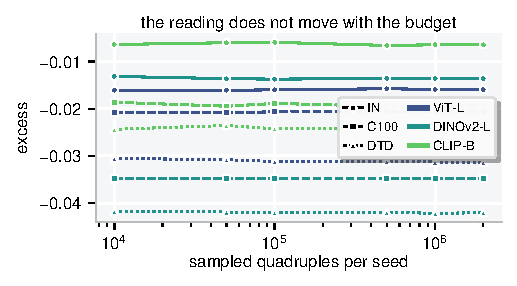
\includegraphics[width=0.62\linewidth]{figures/fig_budget_final.pdf}
\caption{\textbf{The reading does not move with the quadruple budget.} Excess against the number of sampled quadruples per seed, one line per cell: 3 backbones on ImageNet, CIFAR-100 and DTD. % expR72_budget_record.csv
}
\label{fig:budget}
\end{figure}
% prov: expR72_budget_record.csv, expR72_budget_record_summary.csv, expR32_centroid_bootstrap.csv, expR59_imagenet_bootstrap_summary.csv, expR66_joint_sensitivity_summary.csv, expR60_c_sweep_record.csv, analysis4_finetuning.csv, e1_delta_by_layer.csv
\begin{table}[tbp]
\centering
\scriptsize
\setlength{\tabcolsep}{2.4pt}
\begingroup
\noindent\textbf{(a) Quadruple budget: the excess at $10^4$ to $2{\times}10^6$ sampled quadruples per seed under the record (Haar null, p99.9, 200 replicates).}\par\vspace{1.5pt}
\setlength{\tabcolsep}{2.2pt}
\begin{tabular}{llccccccc|cc}
\toprule
model & data & protocol & $10^4$ & $5{\times}10^4$ & $10^5$ & $5{\times}10^5$ & $10^6$ & $2{\times}10^6$ & drift ($\ge10^5$) & drift/s.d. \\
\midrule
ViT-L & IN & record & $-0.0161$ & $-0.0161$ & $-0.0160$ & $-0.0157$ & $-0.0159$ & $-0.0159$ & $0.0002$ & 0.07 \\
DINOv2-L & IN & record & $-0.0131$ & $-0.0136$ & $-0.0137$ & $-0.0135$ & $-0.0136$ & $-0.0136$ & $0.0002$ & 0.38 \\
CLIP-B & IN & record & $-0.0063$ & $-0.0060$ & $-0.0059$ & $-0.0065$ & $-0.0064$ & $-0.0064$ & $0.0007$ & 0.13 \\
ViT-L & C100 & record & $-0.0208$ & $-0.0208$ & $-0.0206$ & $-0.0205$ & $-0.0205$ & $-0.0205$ & $0.0002$ & 0.03 \\
DINOv2-L & C100 & record & $-0.0348$ & $-0.0348$ & $-0.0348$ & $-0.0348$ & $-0.0347$ & $-0.0347$ & $0.0001$ & 0.07 \\
CLIP-B & C100 & record & $-0.0186$ & $-0.0195$ & $-0.0188$ & $-0.0195$ & $-0.0194$ & $-0.0194$ & $0.0006$ & 0.10 \\
ViT-L & DTD & record & $-0.0305$ & $-0.0308$ & $-0.0312$ & $-0.0311$ & $-0.0313$ & $-0.0313$ & $0.0002$ & 0.05 \\
DINOv2-L & DTD & record & $-0.0418$ & $-0.0419$ & $-0.0421$ & $-0.0420$ & $-0.0422$ & $-0.0420$ & $0.0002$ & 0.06 \\
CLIP-B & DTD & record & $-0.0243$ & $-0.0235$ & $-0.0242$ & $-0.0240$ & $-0.0243$ & $-0.0242$ & $0.0003$ & 0.05 \\
ViT-L & C100 & \multicolumn{9}{l}{centroid bootstrap: excess $-0.0493$, s.d.\ $0.0029$ (30 resamples of the per-class images, 500 images/class)} \\
DINOv2-L & C100 & \multicolumn{9}{l}{centroid bootstrap: excess $-0.0493$, s.d.\ $0.0022$ (30 resamples of the per-class images, 500 images/class)} \\
DINOv2-G & C100 & \multicolumn{9}{l}{centroid bootstrap: excess $-0.0778$, s.d.\ $0.0020$ (30 resamples of the per-class images, 500 images/class)} \\
CLIP-B & C100 & \multicolumn{9}{l}{centroid bootstrap: excess $-0.0476$, s.d.\ $0.0017$ (30 resamples of the per-class images, 500 images/class)} \\
ViT-L & DTD & \multicolumn{9}{l}{centroid bootstrap: excess $-0.0803$, s.d.\ $0.0049$ (30 resamples of the per-class images, 80 images/class)} \\
DINOv2-L & DTD & \multicolumn{9}{l}{centroid bootstrap: excess $-0.0878$, s.d.\ $0.0048$ (30 resamples of the per-class images, 80 images/class)} \\
DINOv2-G & DTD & \multicolumn{9}{l}{centroid bootstrap: excess $-0.0863$, s.d.\ $0.0051$ (30 resamples of the per-class images, 80 images/class)} \\
CLIP-B & DTD & \multicolumn{9}{l}{centroid bootstrap: excess $-0.0581$, s.d.\ $0.0054$ (30 resamples of the per-class images, 80 images/class)} \\
\bottomrule
\end{tabular}
\par\vspace{5pt}
\endgroup
\caption{\textbf{The excess is budget-stable, the genuine count survives resampling and estimator noise, the reading follows the hierarchy of the labels rather than their number, and training moves it.} (a) Excess against the quadruple budget for nine cells; drift = range of the record excess over budgets $\ge10^5$, divided by the excess's spread in the last column; under the record every sign holds at every budget. (b) Bootstrap of the ImageNet excess over resampled images per class: the bootstrap s.d.\ is at most 0.0011 and every resample of every backbone is sign-negative. % expR72_budget_record.csv, expR32_centroid_bootstrap.csv, expR59_imagenet_bootstrap_summary.csv
}
\label{tab:q8-robust}
\end{table}
\begin{table}[tbp]\ContinuedFloat
\centering
\scriptsize
\setlength{\tabcolsep}{2.4pt}
\begingroup
\noindent\textbf{(b) ImageNet centroid bootstrap under the record: 30 resamples of the 100 training images per class (20 null replicates per resample).}\par\vspace{1.5pt}
\footnotesize
\setlength{\tabcolsep}{4pt}
\begin{tabular}{lcccc}
\toprule
model & excess (reference) & bootstrap mean & bootstrap s.d. & fraction negative \\
\midrule
ViT-T & $-0.0055$ & $-0.0051$ & $0.0011$ & 1.00 \\
ViT-S & $-0.0126$ & $-0.0122$ & $0.0007$ & 1.00 \\
ViT-B & $-0.0165$ & $-0.0160$ & $0.0006$ & 1.00 \\
ViT-L & $-0.0160$ & $-0.0160$ & $0.0004$ & 1.00 \\
\midrule
DINO-B & $-0.0209$ & $-0.0208$ & $0.0003$ & 1.00 \\
DINOv2-S & $-0.0164$ & $-0.0162$ & $0.0004$ & 1.00 \\
DINOv2-B & $-0.0167$ & $-0.0164$ & $0.0002$ & 1.00 \\
DINOv2-L & $-0.0136$ & $-0.0134$ & $0.0001$ & 1.00 \\
DINOv2-G & $-0.0080$ & $-0.0083$ & $0.0004$ & 1.00 \\
\midrule
CLIP-B & $-0.0068$ & $-0.0069$ & $0.0009$ & 1.00 \\
CLIP-L & $-0.0094$ & $-0.0095$ & $0.0006$ & 1.00 \\
SigLIP-B & $-0.0080$ & $-0.0081$ & $0.0006$ & 1.00 \\
\bottomrule
\end{tabular}
\par\vspace{5pt}
\endgroup
\caption{(continued)}
\end{table}
\begin{table}[tbp]\ContinuedFloat
\centering
\scriptsize
\setlength{\tabcolsep}{2.4pt}
\begingroup
\noindent\textbf{(c) Joint sensitivity of the genuine count: $z_{\text{joint}}$ against null, bootstrap and estimator noise, and (in parentheses) the number of the 30 centroid resamples in which the cell is genuine.}\par\vspace{1.5pt}
\setlength{\tabcolsep}{2.6pt}
\begin{tabular}{lcccccc}
\toprule
model & IN & C100 & C10 & DTD & FMNIST & MNIST \\
\midrule
ViT-T & $-1.1$ (0)$^{\circ}$ & $-0.7$ (0)$^{\circ}$ & $-1.1$ (0)$^{\circ}$ & $-2.0$ (13)$^{\dagger}$ & $+0.9$ (0)$^{\circ}$ & $-1.0$ (0)$^{\circ}$ \\
ViT-S & $-3.6$ (30) & $-0.0$ (0)$^{\circ}$ & $-2.7$ (30) & $-3.1$ (30) & $-1.7$ (30)$^{\dagger}$ & $-1.3$ (0)$^{\circ}$ \\
ViT-B & $-5.2$ (30) & $+0.8$ (0)$^{\circ}$ & $-2.4$ (30) & $-4.0$ (30) & $-2.1$ (30) & $-0.6$ (0)$^{\circ}$ \\
ViT-L & $-5.0$ (30) & $-4.0$ (30) & $-2.8$ (30) & $-6.4$ (30) & $-2.5$ (30) & $-1.6$ (0)$^{\circ}$ \\
\midrule
DINO-B & $-8.9$ (30) & $-7.6$ (30) & $-2.7$ (30) & $-4.5$ (30) & $-0.3$ (0)$^{\circ}$ & $-1.5$ (0)$^{\circ}$ \\
DINOv2-S & $-15.9$ (30) & $-9.7$ (30) & $-2.8$ (30) & $-3.2$ (30) & $-1.6$ (30)$^{\circ}$$^{\ddagger}$ & $-0.2$ (0)$^{\circ}$ \\
DINOv2-B & $-31.6$ (30) & $-14.7$ (30) & $-4.3$ (30) & $-8.1$ (30) & $-2.7$ (30) & $-0.6$ (0)$^{\circ}$ \\
DINOv2-L & $-30.7$ (30) & $-21.6$ (30) & $-4.9$ (30) & $-10.6$ (30) & $-1.8$ (29)$^{\dagger}$ & $-0.5$ (0)$^{\circ}$ \\
DINOv2-G & $-11.5$ (30) & $-28.5$ (30) & $-4.8$ (30) & $-8.2$ (30) & $-2.0$ (30) & $-0.8$ (0)$^{\circ}$ \\
\midrule
CLIP-B & $-1.3$ (0)$^{\circ}$ & $-3.1$ (30) & $-1.8$ (7)$^{\dagger}$ & $-3.5$ (30) & $-1.3$ (0)$^{\circ}$ & $-0.0$ (0)$^{\circ}$ \\
CLIP-L & $-2.1$ (12)$^{\dagger}$ & $-3.5$ (30) & $-2.0$ (30)$^{\dagger}$ & $-4.3$ (30) & $-1.5$ (0)$^{\circ}$ & $-0.4$ (0)$^{\circ}$ \\
SigLIP-B & $-1.7$ (0)$^{\circ}$ & $-4.3$ (30) & $-2.6$ (30) & $-4.1$ (30) & $-2.0$ (30)$^{\dagger}$ & $-1.9$ (30)$^{\dagger}$ \\
\bottomrule
\end{tabular}
\par\vspace{5pt}
\endgroup
\caption{(continued) (c) Per cell: $z_{\text{joint}} = \text{excess}/\sqrt{\sigma_{\text{null}}^2+\sigma_{\text{boot}}^2+\sigma_{\text{est}}^2}$ and the number of resamples in which the cell is genuine under BH over the 72 cells; $^{\circ}$: not genuine in the record; $^{\dagger}$: record-genuine but failing one of the two criteria ($z_{\text{joint}}\le-2$, genuine in $\ge27$ of 30); $^{\ddagger}$: not record-genuine but passing one. Counts: record 49/72 (18/24); $z_{\text{joint}}\le-2$: 42/72 (18/24); genuine in $\ge27$ of 30 resamples: 47/72 (17/24). (d) Class-count control under the record (means over subset seeds); ``below'' = subset seeds whose real value lies below the null at uncorrected $p\le0.05$; NC adv = prototype-classifier advantage of the Poincar\'{e} readout in pp. (e) Raw $\delta$ within architecture: fine-tuning on a task without class hierarchy raises it and it falls across transformer depth. % expR66_joint_sensitivity_summary.csv, expR60_c_sweep_record.csv, analysis4_finetuning.csv, e1_delta_by_layer.csv
}
\end{table}
\begin{table}[tbp]\ContinuedFloat
\centering
\scriptsize
\setlength{\tabcolsep}{2.4pt}
\begingroup
\noindent\textbf{(d) Class count against hierarchy depth: ImageNet subsets of $C=100$ classes, random (spanning the hierarchy) or WordNet-coherent (siblings, effectively flat), means over five subset seeds; the other values of $C$ are in the sweep file.}\par\vspace{1.5pt}
\footnotesize
\setlength{\tabcolsep}{3.5pt}
\begin{tabular}{lr|cccc|cccc}
\toprule
 & & \multicolumn{4}{c|}{random subsets (span the hierarchy)} & \multicolumn{4}{c}{WordNet-coherent (siblings)} \\
model & $C$ & $\hat\delta_{99.9}$ & excess & below & NC adv & $\hat\delta_{99.9}$ & excess & below & NC adv \\
\midrule
DINOv2-L & 100 & 0.031 & -0.032 & 5/5 & +1.46 & 0.044 & -0.031 & 5/5 & +0.77 \\
\bottomrule
\end{tabular}
\par\vspace{5pt}
\endgroup
\caption{(continued)}
\end{table}
\begin{table}[tbp]\ContinuedFloat
\centering
\scriptsize
\setlength{\tabcolsep}{2.4pt}
\begingroup
\noindent\textbf{(e) Training moves the raw reading within an architecture: one row per intervention.}\par\vspace{1.5pt}
\footnotesize
\setlength{\tabcolsep}{4pt}
\begin{tabular}{llccc}
\toprule
intervention & model & $\delta$ before & $\delta$ after & change \\
\midrule
non-hierarchical fine-tuning & DINOv2-S & $0.095$ & $0.161$ & $+69\%$ \\
across depth (layer 1 $\to$ 12) & DINOv2-B & $0.147$ & $0.058$ & $-61\%$ \\
\bottomrule
\end{tabular}
\par\vspace{5pt}
\endgroup
\caption{(continued)}
\end{table}


\FloatBarrier
\subsection{Is the structure deeper than a star? The hierarchy test}
\label{app:depth}

\paragraph{What this table answers.} The census certifies structure beyond the second moments, and this table asks whether the clusters are arranged hierarchically. Each backbone is read against a matched star under both constructions of the star. The controls follow: the models supervised on leaf labels, a backbone trained in hyperbolic space with its Euclidean twin, a fine-tuned pair and a control that removes the radial part of every offset. A pre-set criterion expecting no intact certification of the leaf and frozen models was not met, because they are aligned.
\paragraph{The certified set under other groupings.} Only ViT-B and ViT-L are certified under every grouping. A flat cloud clustered under the WordNet grouping fires under the balanced grouping in 38 of 50 runs with clusters rotated. A real cloud read under a grouping that is not its own is therefore expected to fire. The frozen ViT-B firing in 7 of 10 there is consistent with that mismatch and is not evidence of hub structure. % expR64b_wn30bal_summary.csv, expR77_positive_control.csv, expR83_flat_balanced_summary.csv

% prov: expR56_depth_variants.csv, expR69_depth_haarhubs_summary.csv, expR64b_wn30bal_summary.csv, expR70_inet1k_supervised.csv, expR52_census_haar_p999_200.csv, expR63_meru_record.csv, expR65_hier_finetune.csv, expR74_decoupling_summary.csv, expR71_meru_radii.csv, expR77_positive_control.csv, expR77_positive_control_verdict.json, expR82_radial_control.csv, expR82_radial_control_summary.csv
\begin{table}[H]
\centering
\scriptsize
\setlength{\tabcolsep}{2.2pt}
\begingroup
\noindent\textbf{(a) The 12 backbones under the star with Gaussian hubs.}\par\vspace{1.5pt}
\setlength{\tabcolsep}{2.2pt}
\begin{tabular}{lcc@{\hspace{5pt}}cccc@{\hspace{5pt}}c}
\toprule
 & C100, $K{=}20$ & \multicolumn{3}{c}{ImageNet, matched star} & bal.\ frame \\
\cmidrule(lr){2-2}\cmidrule(lr){3-5}\cmidrule(lr){6-6}
model & depth ($z$) & $K{=}10$ $z$ & $K{=}30$ depth ($z$) & $K{=}60$ $z$ & real $z$ \\
\midrule
ViT-T & $-0.025$ (-1.43) & $-1.70$ & $-0.018$ (-1.48) & $-2.53$ & $-2.08$ \\
ViT-S & $-0.008$ (-0.51) & $-1.72$ & $-0.028$ (-2.36) & $-1.78$ & $-1.72$ \\
ViT-B & $+0.003$ (+0.23) & $-2.57$ & $-0.033$ (-3.62) & $-2.23$ & $-2.82$ \\
ViT-L & $-0.017$ (-1.49) & $-2.73$ & $-0.033$ (-4.04) & $-4.69$ & $-5.57$ \\
\midrule
DINO-B & $-0.038$ (-4.24) & $-0.62$ & $-0.009$ (-0.94) & $-1.11$ & $-0.98$ \\
DINOv2-S & $-0.020$ (-1.61) & $+0.26$ & $+0.008$ (+0.66) & $+0.61$ & $+0.12$ \\
DINOv2-B & $+0.010$ (+0.94) & $-0.46$ & $-0.016$ (-1.19) & $-0.75$ & $-0.32$ \\
DINOv2-L & $+0.013$ (+1.20) & $-1.20$ & $-0.028$ (-2.39) & $-1.25$ & $-1.70$ \\
DINOv2-G & $-0.007$ (-0.68) & $-1.00$ & $-0.029$ (-1.78) & $-0.48$ & $-0.93$ \\
\midrule
CLIP-B & $-0.024$ (-2.00) & $-1.55$ & $-0.016$ (-1.95) & $-2.10$ & $-1.29$ \\
CLIP-L & $-0.013$ (-2.34) & $-1.26$ & $-0.008$ (-0.83) & $-1.40$ & $-0.68$ \\
SigLIP-B & $-0.021$ (-2.17) & $-0.76$ & $-0.011$ (-0.90) & $-1.66$ & $-1.12$ \\
\bottomrule
\end{tabular}
\par\vspace{2pt}
\endgroup
\caption{\textbf{The hierarchy test certifies that clusters are oriented toward their hubs in a few backbones, and finds no hierarchy among the hubs.} Panels: the 12 backbones under both matched stars, the leaf-label ViTs, a hyperbolic backbone with its Euclidean twin, the trained control and the radial control.
}
\label{tab:q4-depth}
\end{table}
\begin{table}[H]\ContinuedFloat
\centering
\scriptsize
\setlength{\tabcolsep}{2.2pt}
\begingroup
\noindent\textbf{(a$'$) The same backbones under the star whose hubs are a Haar resample of the real hubs (ImageNet, $K{=}30$); last column.}\par\vspace{1.5pt}
\setlength{\tabcolsep}{4pt}
\begin{tabular}{lcccc}
\toprule
model & star B & depth ($z$) & $r_{\text{star}}$ & decoupled $z$ (cert.) \\
\midrule
ViT-T & $+0.0011$ & $-0.0184$ (-1.45) & 0/10 & $-1.69$ $\pm$ $0.28$ (1/10) \\
ViT-S & $+0.0010$ & $-0.0257$ (-2.04) & 0/10 & $-1.30$ $\pm$ $0.19$ (0/10) \\
ViT-B & $+0.0012$ & $-0.0347$ (-3.01) & 0/10 & $-1.40$ $\pm$ $0.25$ (0/10) \\
ViT-L & $+0.0000$ & $-0.0337$ (-3.73) & 0/10 & $-1.61$ $\pm$ $0.19$ (0/10) \\
\midrule
DINO-B & $+0.0002$ & $-0.0092$ (-1.02) & 0/10 & $+1.75$ $\pm$ $0.16$ (0/10) \\
DINOv2-S & $+0.0007$ & $+0.0083$ (+0.71) & 10/10 & $+1.38$ $\pm$ $0.14$ (0/10) \\
DINOv2-B & $+0.0018$ & $-0.0155$ (-1.18) & 0/10 & $+0.41$ $\pm$ $0.11$ (0/10) \\
DINOv2-L & $-0.0007$ & $-0.0267$ (-2.21) & 0/10 & $-0.20$ $\pm$ $0.14$ (0/10) \\
DINOv2-G & $-0.0021$ & $-0.0263$ (-1.50) & 0/10 & $-0.04$ $\pm$ $0.07$ (0/10) \\
\midrule
CLIP-B & $+0.0012$ & $-0.0171$ (-1.48) & 1/10 & $-1.25$ $\pm$ $0.09$ (0/10) \\
CLIP-L & $+0.0018$ & $-0.0090$ (-0.74) & 2/10 & $-0.88$ $\pm$ $0.22$ (0/10) \\
SigLIP-B & $+0.0024$ & $-0.0121$ (-0.78) & 1/10 & $-0.84$ $\pm$ $0.18$ (0/10) \\
\bottomrule
\end{tabular}
\par\vspace{2pt}
\endgroup
\caption{(continued)}
\end{table}
\begin{table}[H]\ContinuedFloat
\centering
\scriptsize
\setlength{\tabcolsep}{2.2pt}
\begingroup
\noindent\textbf{(b) Two ViT-B/16 supervised on ImageNet-1k leaf labels only, through the census protocol, against the IN-21k census backbone.}\par\vspace{1.5pt}
\setlength{\tabcolsep}{4pt}
\begin{tabular}{lcccc}
\toprule
model & IN excess ($r$) & C100 excess ($r$) & depth, Gaussian hubs ($z$) & depth, Haar hubs ($z$) \\
\midrule
DeiT-B, IN-1k & $-0.0073$ (200) & $-0.0257$ (200) & $-0.0213$ (-1.26) & $-0.0197$ (-1.21) \\
ViT-B, augreg, IN-1k & $-0.0070$ (199) & $-0.0117$ (187) & $-0.0249$ (-3.03) & $-0.0290$ (-2.65) \\
ViT-B, augreg, IN-21k (census) & $-0.0162$ (200) & $+0.0057$ (43) & $-0.0335$ (-3.62) & $-0.0347$ (-3.01) \\
\bottomrule
\end{tabular}
\par\vspace{2pt}
\endgroup
\caption{(continued)}
\end{table}
\begin{table}[H]\ContinuedFloat
\centering
\scriptsize
\setlength{\tabcolsep}{2.2pt}
\noindent\textbf{(c) A hyperbolic backbone and its Euclidean twin under the census and the hierarchy test.}\par\vspace{1.5pt}
\begin{tabular}{llccc@{\hspace{8pt}}ccc}
\toprule
 & & \multicolumn{3}{c}{CIFAR-100 ($K{=}20$, $n{=}100$: false alarms uncontrolled)} & \multicolumn{3}{c}{ImageNet ($K{=}30$, $n{=}1000$: false alarms controlled)} \\
\cmidrule(lr){3-5}\cmidrule(lr){6-8}
model & input & exc.\ ($r$) & $\hat\delta_{99.9}$ nat./Eucl. & depth $z$ & exc.\ ($r$) & $\hat\delta_{99.9}$ nat./Eucl. & depth $z$ \\
\midrule
MERU ViT-S & images & $-0.020$ (199) & $0.117$/$0.117$ & $-1.52$ & $-0.008^{\circ}$ (186) & $0.088$/$0.088$ & $-1.54$ \\
CLIP ViT-S & images & $-0.028$ (200) & $0.106$/$0.107$ & $-3.95$ & $-0.006^{\circ}$ (171) & $0.110$/$0.088$ & $-1.85$ \\
MERU ViT-B & images & $-0.020$ (200) & $0.114$/$0.114$ & $-2.16$ & $-0.010$ (196) & $0.087$/$0.087$ & $-0.86$ \\
CLIP ViT-B & images & $-0.030$ (200) & $0.105$/$0.103$ & $-3.28$ & $-0.009^{\circ}$ (187) & $0.107$/$0.085$ & $-0.99$ \\
MERU ViT-L & images & $-0.012^{\circ}$ (195) & $0.118$/$0.118$ & $-0.29$ & $-0.007^{\circ}$ (184) & $0.088$/$0.088$ & $-0.52$ \\
CLIP ViT-L & images & $-0.016$ (199) & $0.123$/$0.112$ & $-1.68$ & $-0.010$ (197) & $0.104$/$0.084$ & $-1.21$ \\
\midrule
MERU ViT-S & prompts & $-0.022$ (200) & $0.086$/$0.086$ & $-0.67$ & $-0.003^{\circ}$ (155) & $0.085$/$0.086$ & $+0.02$ \\
CLIP ViT-S & prompts & $-0.023$ (200) & $0.085$/$0.082$ & $-0.78$ & $+0.006^{\circ}$ (15) & $0.093$/$0.087$ & $+0.82$ \\
MERU ViT-B & prompts & $-0.012$ (200) & $0.096$/$0.096$ & $-0.70$ & $-0.001^{\circ}$ (132) & $0.089$/$0.090$ & $+0.76$ \\
CLIP ViT-B & prompts & $-0.017$ (200) & $0.094$/$0.088$ & $+0.31$ & $+0.008^{\circ}$ (2) & $0.100$/$0.092$ & $+0.18$ \\
MERU ViT-L & prompts & $-0.006^{\circ}$ (190) & $0.102$/$0.102$ & $+0.58$ & $+0.001^{\circ}$ (75) & $0.093$/$0.093$ & $+0.52$ \\
CLIP ViT-L & prompts & $-0.012$ (200) & $0.098$/$0.092$ & $+0.48$ & $+0.006^{\circ}$ (5) & $0.101$/$0.092$ & $+0.39$ \\
\bottomrule
\end{tabular}
\par\vspace{2pt}
\caption{(continued)}
\end{table}
\begin{table}[H]\ContinuedFloat
\centering
\scriptsize
\setlength{\tabcolsep}{2.2pt}
\begingroup
\noindent\textbf{(d) A trained positive control: leaf cross-entropy against leaf plus hierarchical, 2 seeds, identical batches.}\par\vspace{1.5pt}
\footnotesize
\setlength{\tabcolsep}{3pt}
\begin{tabular}{lccccc}
\toprule
ViT-B/16 & excess ($r$) & $z$, WordNet-30 & dec.\ $z$ (cert.) & $z$, balanced & dec.\ $z$ (cert.) \\
\midrule
frozen (census) & $-0.0162$ (200) & $-3.62$ & $-1.40$ (0.0) & $-2.82$ & $-2.10$ (0.7) \\
leaf cross-entropy, seed 0 & $-0.0243$ (200) & $-2.45$ & $-0.72$ (0.0) & $-2.09$ & $-1.38$ (0.0) \\
leaf + hierarchical, seed 0 & $-0.0293$ (200) & $-2.97$ & $-2.38$ (1.0) & $-3.57$ & $-3.51$ (1.0) \\
leaf cross-entropy, seed 1 & $-0.0242$ (200) & $-3.18$ & $-2.02$ (0.6) & $-2.94$ & $-3.02$ (1.0) \\
leaf + hierarchical, seed 1 & $-0.0295$ (200) & $-4.22$ & $-2.63$ (1.0) & $-5.82$ & $-3.44$ (1.0) \\
\bottomrule
\end{tabular}
\par\vspace{2pt}
\endgroup
\caption{(continued)}
\end{table}
\begin{table}[H]\ContinuedFloat
\centering
\scriptsize
\setlength{\tabcolsep}{2.2pt}
\begingroup
\noindent\textbf{(e) Radial control: centroids normalized, offsets stripped of their radial part.}\par\vspace{1.5pt}
\footnotesize
\setlength{\tabcolsep}{3pt}
\begin{tabular}{lccc|ccc}
\toprule
& \multicolumn{3}{c|}{L2-normalized} & \multicolumn{3}{c}{radial component removed} \\
model & $z$ aniso & $z$ Haar-hub & decoupled $z$ (cert.) & $z$ aniso & $z$ Haar-hub & decoupled $z$ (cert.) \\
\midrule
ViT-T & $+0.27$ & $-0.17$ & $-0.78$ (0.0) & $-2.06$ & $-2.07$ & $-1.74$ (0.3) \\
ViT-S & $-0.76$ & $-0.93$ & $-1.16$ (0.0) & $-2.26$ & $-2.08$ & $-1.25$ (0.0) \\
ViT-B & $-2.45$ & $-2.52$ & $-0.57$ (0.0) & $-3.60$ & $-3.57$ & $-1.40$ (0.0) \\
ViT-L & $-2.00$ & $-2.23$ & $-1.41$ (0.1) & $-3.99$ & $-3.47$ & $-1.47$ (0.0) \\
\midrule
DINO-B & $+0.82$ & $+0.95$ & $+2.00$ (0.0) & $-1.61$ & $-1.89$ & $+1.91$ (0.0) \\
DINOv2-S & $+1.27$ & $+1.38$ & $+1.28$ (0.0) & $+0.61$ & $+0.58$ & $+1.43$ (0.0) \\
DINOv2-B & $-0.07$ & $-0.01$ & $+1.28$ (0.0) & $-1.18$ & $-1.19$ & $+0.46$ (0.0) \\
DINOv2-L & $-0.46$ & $-0.50$ & $+0.89$ (0.0) & $-2.59$ & $-2.28$ & $-0.01$ (0.0) \\
DINOv2-G & $-0.78$ & $-0.76$ & $+0.88$ (0.0) & $-1.75$ & $-1.66$ & $+0.11$ (0.0) \\
\midrule
CLIP-B & $-1.42$ & $-0.93$ & $-1.38$ (0.0) & $-1.53$ & $-1.06$ & $-1.19$ (0.0) \\
CLIP-L & $-1.57$ & $-1.12$ & $-0.82$ (0.0) & $-1.05$ & $-0.89$ & $-0.92$ (0.0) \\
SigLIP-B & $-1.13$ & $-0.88$ & $-0.51$ (0.0) & $-1.12$ & $-1.07$ & $-0.89$ (0.0) \\
\bottomrule
\end{tabular}
\par\vspace{2pt}
\endgroup
\caption{(continued)}
\end{table}


\FloatBarrier
\subsection{How much depth can the test see? Power on synthetic and planted hierarchies}
\label{app:power}
\paragraph{What this table answers.} A negative verdict is worth reading only where the test can see. Here hierarchies of known strength are planted in real and synthetic clouds and the test is run again, which gives its power; flat clouds are read the same way, which gives its false alarms. The power depends on how quiet the cloud is, so it is reported per backbone.
\begin{figure}[H]
\centering
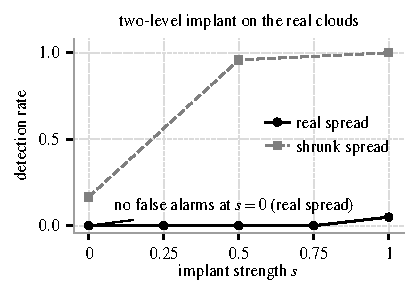
\includegraphics[width=0.5\linewidth]{figures/fig_implant_final.pdf}
\caption{\textbf{A planted two-level tree on the real ImageNet clouds is missed at the real within-cluster spread and detected once the spread is shrunk.} Detection rate at $z\le-2$ against planted-tree strength $s$ with the real within-cluster spread (solid) and shrunk (dashed): at full strength 0.05 against 1.00, and 0.00 at $s=0$ with the real spread. % expR64b_wn30.csv
}
\label{fig:implant}
\end{figure}
\begin{figure}[H]
\centering
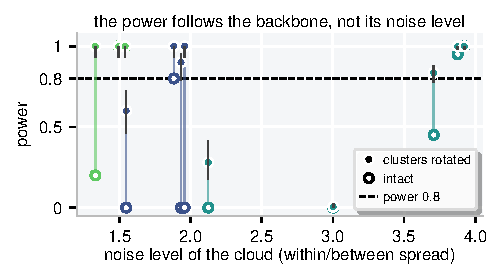
\includegraphics[width=0.62\linewidth]{figures/fig_power_final.pdf}
\caption{\textbf{The power follows the backbone, not the noise level of its cloud.} Power against the within/between spread, intact (hollow) and with clusters rotated (filled); whiskers: 95 per cent intervals over 50 runs per backbone, 200 for the DINOv2 family. % expR81_deep_per_backbone_summary.csv, expR64b_wn30_summary.csv
}
\label{fig:power}
\end{figure}
% prov: expR55_depth_power.csv, expR55b_depth_power_leafframe.csv, expR64b_wn30.csv, expR64b_wn30_summary.csv, expR64b_wn30bal_summary.csv, expR67_frame_choice.json, expR69_depth_haarhubs_summary.csv, expR80_implanted_alignment.csv, expR80_decision.csv, expR79_synthetic_deep_poincare.csv, expR81_deep_per_backbone.csv, expR81_deep_per_backbone_summary.csv, expR83_flat_balanced.csv, expR83_flat_balanced_summary.csv
\begin{table}[H]
\centering
\scriptsize
\setlength{\tabcolsep}{2pt}
\begingroup
\footnotesize
\setlength{\tabcolsep}{4pt}
\begin{tabular}{lccccc}
\toprule
cloud & seed & $d$ & excess ($r$) & depth $z$ & decoupled $z$ (cert.) \\
\midrule
three-level hierarchy, ViT-L spectrum & 0 & 1024 & $-0.0081$ (199) & $-1.80$ & $-4.82$ $\pm$ 0.73 (1.0) \\
three-level hierarchy, ViT-L spectrum & 1 & 1024 & $-0.0095$ (199) & $-2.45$ & $-4.44$ $\pm$ 0.58 (1.0) \\
three-level hierarchy, ViT-L spectrum & 2 & 1024 & $-0.0090$ (199) & $-2.38$ & $-4.19$ $\pm$ 0.60 (1.0) \\
three-level hierarchy, ViT-L spectrum & 3 & 1024 & $-0.0099$ (199) & $-2.08$ & $-4.48$ $\pm$ 0.67 (1.0) \\
three-level hierarchy, ViT-L spectrum & 4 & 1024 & $-0.0090$ (199) & $-2.20$ & $-4.28$ $\pm$ 0.54 (1.0) \\
\midrule
flat control, ViT-L spectrum & 0 & 1024 & $-0.0198$ (200) & $-0.08$ & $-1.61$ $\pm$ 0.27 (0.1) \\
flat control, ViT-L spectrum & 1 & 1024 & $-0.0202$ (200) & $-0.32$ & $-1.61$ $\pm$ 0.31 (0.1) \\
flat control, ViT-L spectrum & 2 & 1024 & $-0.0196$ (200) & $-0.20$ & $-1.76$ $\pm$ 0.37 (0.2) \\
flat control, ViT-L spectrum & 3 & 1024 & $-0.0197$ (200) & $-0.69$ & $-1.74$ $\pm$ 0.33 (0.2) \\
flat control, ViT-L spectrum & 4 & 1024 & $-0.0192$ (200) & $-0.27$ & $-1.68$ $\pm$ 0.39 (0.2) \\
\midrule
WordNet Poincar\'e, $d{=}10$ & 0 & 10 & $+0.0830$ (0) & $+2.36$ & $+0.32$ $\pm$ 0.58 (0.0) \\
WordNet Poincar\'e, $d{=}50$ & 0 & 50 & $+0.0354$ (0) & $+1.53$ & $-2.22$ $\pm$ 0.65 (0.6) \\
\bottomrule
\end{tabular}
\par\vspace{2pt}
\endgroup
\caption{\textbf{A deep hierarchy at the real noise level is detected, and a flat control is not.} Synthetic clouds with ViT-L's spectrum and ratio: the depth $z$ intact and decoupled for the hierarchy and for the flat control.
}
\label{tab:q5-power}\label{tab:q5-power-d}
\end{table}


\FloatBarrier
\subsection{Is the island real? The tree map and the within-model ceiling}
\label{app:treemap}

\paragraph{What this table answers.} Trees of different models are compared as objects, without labels. The comparison depends on the cut, so the first table gives the diagnostics of every admissible configuration and the criterion that selects one. The ceiling any cross-model agreement can reach is what two resamples of the same model agree on, 0.90 on triplets; Figure~\ref{fig:treemap}b carries it as the band behind each model.
% prov: exp22_tree_similarity_imagenet.npz, exp23_treemap_controls.npz, exp23_config_diagnostics.json, expR58_treemap_cutfree_summary.csv, expR84_tree_ceiling.csv, expR84_tree_ceiling_summary.csv
\begin{table}[H]
\centering
\scriptsize
\setlength{\tabcolsep}{3pt}
\begingroup
\setlength{\tabcolsep}{3pt}
\begin{tabular}{ll|ccc}
\toprule
dataset & configuration & ARI at the cut & cophenetic corr. & triplet agreement \\
\midrule
ImageNet & euclid-average (deg.) & 0.03 / 0.64 & 0.36 / 0.80 & 0.47 / 0.74 \\
ImageNet & euclid-complete (deg.) & 0.03 / 0.44 & 0.20 / 0.66 & 0.41 / 0.65 \\
ImageNet & euclid-ward & 0.16 / 0.53 & 0.62 / 0.84 & 0.67 / 0.85 \\
ImageNet & cosine-average (selected) & 0.39 / 0.48 & 0.48 / 0.78 & 0.77 / 0.76 \\
ImageNet & cosine-complete & 0.13 / 0.49 & 0.18 / 0.72 & 0.36 / 0.71 \\
ImageNet & cosine-ward & 0.17 / 0.55 & 0.59 / 0.85 & 0.69 / 0.86 \\
\midrule
CIFAR-100 & euclid-average (deg.) & 0.00 / 0.57 & 0.15 / 0.78 & 0.41 / 0.74 \\
CIFAR-100 & euclid-complete (deg.) & 0.17 / 0.54 & 0.23 / 0.72 & 0.41 / 0.66 \\
CIFAR-100 & euclid-ward & 0.37 / 0.63 & 0.63 / 0.77 & 0.70 / 0.79 \\
CIFAR-100 & cosine-average (deg.) & 0.30 / 0.58 & 0.42 / 0.72 & 0.51 / 0.64 \\
CIFAR-100 & cosine-complete (selected) & 0.39 / 0.63 & 0.46 / 0.64 & 0.50 / 0.61 \\
CIFAR-100 & cosine-ward & 0.56 / 0.61 & 0.74 / 0.73 & 0.76 / 0.76 \\
\bottomrule
\end{tabular}
\par\vspace{2pt}
\endgroup
\caption{\textbf{The self-supervised models sit apart on distances, not on topology.} The three agreement measures for DINOv2 against the supervised and contrastive models, each written as against those models over within them.
}
\label{tab:q6-treemap}\label{tab:q6-treemap-b}
\end{table}


\FloatBarrier
\subsection{Is local structure shared? Permutation-calibrated agreement}
\label{app:local}
\paragraph{What this table answers.} Two models can place classes in the same neighborhoods and still disagree on distances. This table calibrates both readings against permutations of the class labels, so agreement is counted only where a shuffled pairing would not reach it.
\paragraph{Models share neighborhoods, not metrics.} Permutation-calibrated mutual-kNN agreement and centroid CKA survive across all 66 model pairs, and the Poincar\'{e} metric improves neither \citep{groger2026aristotelian} (Table~\ref{tab:q13-local}). % exp21b_local_global_K200.csv
% prov: exp21b_local_global_K200.csv
\begin{table}[H]
\centering
\footnotesize
\setlength{\tabcolsep}{3pt}
\begin{tabular}{lcccccc}
\toprule
measure & raw & null mean & $\tau_{0.05}$ & calibrated & null-centered & pairs $p<0.05$ \\
\midrule
mutual-kNN ($k{=}10$), Euclidean & $0.472$ & $0.010$ & $0.015$ & $0.464$ & $0.462$ & 66/66 \\
mutual-kNN, Poincar\'e & $0.425$ & $0.010$ & $0.019$ & $0.414$ & $0.415$ & 66/66 \\
linear CKA, Euclidean & $0.633$ & $0.108$ & $0.111$ & $0.577$ & $0.524$ & 66/66 \\
linear CKA, Poincar\'e & $0.640$ & $0.108$ & $0.111$ & $0.586$ & $0.532$ & 66/66 \\
\bottomrule
\end{tabular}
\par\vspace{2pt}
\caption{\textbf{Cross-model agreement survives permutation calibration.} Columns: the raw measure, the null mean, the calibration threshold, the calibrated value and the number of model pairs that survive, for mutual-kNN agreement and for centroid CKA.
}
\label{tab:q13-local}
\end{table}


\FloatBarrier
\subsection{Whose taxonomy? WordNet alignment, superclass recovery, DBpedia and HierarCaps}
\label{app:wordnet}
\label{app:hierarcaps}
\paragraph{What this table answers.} Here the trees are compared with a human taxonomy instead of with each other. The first two tables use WordNet on ImageNet and the coarse labels of CIFAR-100. The last two repeat the reading on an ontology built independently of WordNet and on a set of caption chains with no class set, so the recovery is not circular.
% prov: exp3_alignment.csv, exp28_recovery_per_config.csv, exp8_p1_recovery.csv, exp1_delta_controls.csv, exp8_p6_pooling.csv, expR70_inet1k_supervised.csv, exp14_dbpedia.csv, expR61_dbpedia_record.csv, exp27_dbpedia_treemap.json, exp16_hierarcaps.csv
\begin{table}[H]
\centering
\scriptsize
\setlength{\tabcolsep}{2.6pt}
\begingroup
\footnotesize
\setlength{\tabcolsep}{4pt}
\begin{tabular}{lcccc|c}
\toprule
 & \multicolumn{4}{c|}{Spearman $\rho$, inter-centroid vs WordNet distance} & raw $\hat\delta$ of \\
model & $\rho_{\text{WN}}$ & shuffle & Gaussian & single image & WordNet / random groups \\
\midrule
ViT-T & $+0.52$ & $+0.02$ & $+0.01$ & -- & 0.146 / 0.159 \\
ViT-S & $+0.50$ & $+0.00$ & $-0.00$ & -- & 0.110 / 0.130 \\
ViT-B & $+0.49$ & $+0.03$ & $+0.01$ & -- & 0.092 / 0.120 \\
ViT-L & $+0.53$ & $+0.01$ & $+0.03$ & $+0.25$ & 0.104 / 0.117 \\
\midrule
DINO-B & $+0.36$ & $-0.01$ & $-0.01$ & -- & 0.084 / 0.117 \\
DINOv2-S & $+0.22$ & $+0.01$ & $+0.01$ & -- & 0.077 / 0.100 \\
DINOv2-B & $+0.18$ & $-0.01$ & $+0.01$ & -- & 0.068 / 0.069 \\
DINOv2-L & $+0.18$ & $-0.00$ & $-0.03$ & $+0.08$ & 0.060 / 0.058 \\
DINOv2-G & $+0.20$ & $-0.03$ & $-0.01$ & $+0.03$ & 0.054 / 0.056 \\
\midrule
CLIP-B & $+0.57$ & $+0.00$ & $+0.01$ & -- & 0.126 / 0.174 \\
CLIP-L & $+0.59$ & $+0.01$ & $+0.03$ & $+0.26$ & 0.117 / 0.162 \\
SigLIP-B & $+0.58$ & $-0.01$ & $+0.01$ & -- & 0.118 / 0.158 \\
\midrule
DeiT-B (IN-1k) & $+0.08$ & $+0.01$ & -- & -- & -- \\
ViT-B (augreg, IN-1k) & $+0.52$ & $+0.01$ & -- & -- & -- \\
\bottomrule
\end{tabular}
\par\vspace{2pt}
\endgroup
\caption{\textbf{Agreement with the human taxonomy follows supervision and recipe.} Per backbone on ImageNet: the correlation between inter-centroid and WordNet distances, the same under shuffled labels, a Gaussian cloud and single images, and the raw reading of WordNet against random groups.
}
\label{tab:q7-wordnet}
\end{table}
\begin{table}[H]
\centering
\scriptsize
\setlength{\tabcolsep}{2.6pt}
\begingroup
\setlength{\tabcolsep}{2.5pt}
\begin{tabular}{lcc|cccc|ccc}
\toprule
 & \multicolumn{2}{c|}{supremum, Haar} & \multicolumn{4}{c|}{census} & & & \\
model & $\hat\delta_{\max}$ & excess & $\hat\delta_{99.9}$ & excess & $r$/200 & $p$ & trip.\ & NC H$-$R & FS H$-$R \\
\midrule
BGE-base & 0.122 & -0.032 & 0.082 & -0.021 & 200 & 0.005 & 0.89 & -0.59 & +0.05$\pm$0.05 \\
E5-base & 0.127 & -0.028 & 0.086 & -0.017 & 200 & 0.005 & 0.89 & -0.43 & +0.04$\pm$0.03 \\
GTE-base & 0.132 & -0.024 & 0.088 & -0.017 & 200 & 0.005 & 0.89 & -0.82 & +0.08$\pm$0.06 \\
\bottomrule
\end{tabular}
\par\vspace{2pt}
\endgroup
\caption{\textbf{The recovery is not WordNet circularity.} On DBpedia Classes, an ontology built independently: the reading, the excess, the triplet agreement and the metric gains per text embedder. $r$/200: replicates above the real value.
}
\label{tab:q7-wordnet-c}
\end{table}
\begin{table}[H]
\centering
\scriptsize
\setlength{\tabcolsep}{2.6pt}
\begingroup
\footnotesize
\setlength{\tabcolsep}{4pt}
\begin{tabular}{lcccccc}
\toprule
model & $\rho$(level, radius) & \% monotone & trip.\ L1 & trip.\ L2 & $\hat\delta$ leaves & excess \\
\midrule
BGE-base & +0.80$\pm$0.31 & 49.6 & 0.88 & 0.97 & 0.130 & +0.003 \\
E5-base & +0.87$\pm$0.19 & 53.9 & 0.90 & 0.97 & 0.139 & +0.010 \\
GTE-base & +0.47$\pm$0.55 & 24.0 & 0.90 & 0.97 & 0.135 & +0.006 \\
CLIP-B & +0.64$\pm$0.43 & 27.2 & 0.86 & 0.95 & 0.123 & -0.011 \\
CLIP-L & +0.51$\pm$0.49 & 18.7 & 0.86 & 0.96 & 0.117 & -0.010 \\
SigLIP-B & +0.32$\pm$0.55 & 9.8 & 0.83 & 0.91 & 0.138 & +0.014 \\
\bottomrule
\end{tabular}
\par\vspace{2pt}
\endgroup
\caption{\textbf{A caption hierarchy with no class set reads the same way.} On HierarCaps: the correlation between level and radius, the share of monotone chains, the triplet agreements and the leaf excess per encoder.
}
\label{tab:q7-wordnet-d}
\end{table}


\FloatBarrier
\subsection{Is text the same? The text census under the census reading}
\label{app:textcensus}
\label{app:templates}

\paragraph{What this table answers.} The text census reads the thousand ImageNet class names through language models and sentence embedders. The verdicts follow the recipe and the scale of the model, not its family. Extraction is part of the measurement, so the second table varies batch size and precision on the same prompts.
% prov: expR53_text_haar_p999_200.csv, expR53_text_haar_sup_200.csv, expR53_text_gauss_p999_200.csv, expR48b_text_census200_bs1.csv, expR57_text_cosine_haar_p999_200.csv, exp18_text_nulls.csv, exp4_prompt_variation.csv, exp17_wordnet_prompts.csv, expR49_template_nulls_bs1.csv, expR47_extraction_variance.csv
\begin{table}[H]
\centering
\scriptsize
\setlength{\tabcolsep}{2.5pt}
\begingroup
\setlength{\tabcolsep}{3.5pt}
\begin{tabular}{llrccccccc|cc}
\toprule
 & & & \multicolumn{6}{c|}{record} & \multicolumn{2}{c}{cosine} \\
model & type & $d$ & $\hat\delta_{99.9}$ & excess & exc./null & $r$/200 & $p$ & 2$\times$2 & exc.\ & $r$ \\
\midrule
GPT-2 S & causal LM & 768 & $0.077$ & $-0.013$ & $-15\%$ & 197 & .020 & $\bullet$$\circ$$\bullet$$\circ$ & $+0.000^{\circ}$ & 101 \\
GPT-2 M & causal LM & 1024 & $0.052$ & $-0.005^{\circ}$ & $-9\%$ & 170 & .154 & $\circ$$\circ$$\circ$$\circ$ & $-0.019$ & 200 \\
GPT-2 L & causal LM & 1280 & $0.053$ & $-0.023$ & $-30\%$ & 200 & .005 & $\bullet$$\bullet$$\bullet$$\bullet$ & $-0.016$ & 200 \\
GPT-2 XL & causal LM & 1600 & $0.048$ & $-0.027$ & $-36\%$ & 200 & .005 & $\bullet$$\bullet$$\bullet$$\bullet$ & $-0.018$ & 200 \\
\midrule
Pythia-410M & causal LM & 1024 & $0.067$ & $-0.018$ & $-21\%$ & 200 & .005 & $\bullet$$\bullet$$\bullet$$\bullet$ & $-0.024$ & 200 \\
Pythia-1B & causal LM & 2048 & $0.066$ & $-0.015$ & $-18\%$ & 199 & .010 & $\bullet$$\bullet$$\bullet$$\bullet$ & $-0.026$ & 200 \\
Pythia-2.8B & causal LM & 2560 & $0.066$ & $-0.017$ & $-20\%$ & 200 & .005 & $\bullet$$\bullet$$\bullet$$\bullet$ & $-0.023$ & 200 \\
OLMo-1B & causal LM & 2048 & $0.051$ & $-0.024$ & $-32\%$ & 200 & .005 & $\bullet$$\bullet$$\bullet$$\bullet$ & $-0.032$ & 200 \\
\midrule
BGE-base & embedder & 768 & $0.078$ & $+0.003^{\circ}$ & $+4\%$ & 26 & .871 & $\circ$$\circ$$\circ$$\circ$ & $-0.002^{\circ}$ & 151 \\
BGE-large & embedder & 1024 & $0.078$ & $+0.002^{\circ}$ & $+3\%$ & 49 & .756 & $\circ$$\circ$$\circ$$\circ$ & $-0.003^{\circ}$ & 170 \\
GTE-base & embedder & 768 & $0.076$ & $+0.004^{\circ}$ & $+6\%$ & 11 & .945 & $\circ$$\circ$$\circ$$\circ$ & $+0.001^{\circ}$ & 79 \\
GTE-large & embedder & 1024 & $0.075$ & $+0.003^{\circ}$ & $+3\%$ & 36 & .821 & $\circ$$\circ$$\circ$$\circ$ & $-0.001^{\circ}$ & 131 \\
GTE-Qwen2-1.5B & embedder & 1536 & $0.078$ & $+0.002^{\circ}$ & $+3\%$ & 58 & .711 & $\circ$$\circ$$\circ$$\circ$ & $-0.006$ & 199 \\
E5-base & embedder & 768 & $0.074$ & $+0.004^{\circ}$ & $+6\%$ & 15 & .925 & $\circ$$\circ$$\circ$$\circ$ & $+0.000^{\circ}$ & 97 \\
E5-large & embedder & 1024 & $0.071$ & $+0.002^{\circ}$ & $+3\%$ & 44 & .781 & $\circ$$\circ$$\circ$$\circ$ & $-0.001^{\circ}$ & 119 \\
\bottomrule
\end{tabular}
\par\vspace{2pt}
\endgroup
\caption{\textbf{In text the verdict follows the recipe and the scale.} Per model: dimension, the reading, the excess, the excess as a fraction of the null, the rank, the left-tail $p$ and the cosine reading beside it.
}
\label{tab:q2-text}
\end{table}
\begin{table}[H]
\centering
\scriptsize
\setlength{\tabcolsep}{2.5pt}
\begingroup
\footnotesize
\setlength{\tabcolsep}{4pt}
\begin{tabular}{lcc|cc}
\toprule
& \multicolumn{2}{c|}{GPT-2 M} & \multicolumn{2}{c}{OLMo-1B} \\
batch size & fp32 $\hat\delta$ & fp16 $\hat\delta$ & fp32 $\hat\delta$ & fp16 $\hat\delta$ \\
\midrule
1 (no padding) & $0.0816$ & $0.0817$ & $0.0817$ & $0.0817$ \\
16 & $0.0996$ & $0.0997$ & $0.0817$ & $0.0816$ \\
32 & $0.0905$ & $0.0905$ & $0.0817$ & $0.0817$ \\
\bottomrule
\end{tabular}
\par\vspace{2pt}
\endgroup
\caption{\textbf{Extraction is part of the measurement.} The same thousand prompts under changes of batch size and of precision: the reading per setting for a causal language model of each family.
}
\label{tab:q2-text-c}
\end{table}


\FloatBarrier
\subsection{What follows for practice? The corollary}
\label{app:corollary}
\label{app:familycorr}

\paragraph{What this table answers.} The instrument certifies structure; this table asks what it buys downstream. Accuracies and zero-cost gains are read per cell, then correlated with the raw reading, with the calibrated one and with the hierarchy verdict. The gains are modest and limited to prototype tasks.
\begin{figure}[H]
\centering

\includegraphics[width=0.92\linewidth]{figures/fig_gains_final.pdf}
\caption{\textbf{The zero-cost advantage is small and largest for the self-supervised models.} Best few-shot advantage over the Euclidean metric, averaged over ImageNet, CIFAR-100, CIFAR-10 and DTD, with the metric that collects it; the 10 backbones evaluated, DINO-B and SigLIP-B excluded. % exp2_metric_controls.csv
}
\label{fig:gains}
\end{figure}
\paragraph{The zero-cost metric.} In few-shot learning a fixed-radius Euclidean encoder does at least as well as hyperbolic prototypes \citep{moreira2024hyperbolic} (Table~\ref{tab:q9-corollary}). % exp2b_normalized_stack.csv, exp24_val_metric_selection.csv

% prov: table1_regenerated.csv, exp2_metric_controls.csv, exp2b_normalized_stack.csv, exp13_mcnemar.csv, night/correlation_cis.csv, exp20_null_ztable.csv, expR68_corollary_excess.csv, exp24_val_metric_selection.csv, night/t_sweep.csv
\begin{table}[tbp]
\centering
\scriptsize
\setlength{\tabcolsep}{2.6pt}
\begingroup
\noindent\textbf{(a) Task accuracies and zero-cost metric gains per cell (10 backbones with cached per-dataset features $\times$ 6 datasets).}\par\vspace{1.5pt}
\scriptsize\renewcommand{\arraystretch}{0.88}
\setlength{\tabcolsep}{3pt}
\begin{tabular}{llcccccccc}
\toprule
 & & \multicolumn{2}{c}{NC acc.\ (\%)} & \multicolumn{2}{c}{FS acc.\ (\%)} & \multicolumn{3}{c}{FS advantage over Euclidean (pp)} & McNemar \\
\cmidrule(lr){3-4}\cmidrule(lr){5-6}\cmidrule(lr){7-9}
model & data & Eucl. & Poinc. & Eucl. & Poinc. & cosine & radial map & Poinc.$_{\text{N}}$ $-$ cos & NC H vs R \\
\midrule
ViT-T & IN & 68.1 & 67.2 & 97.5 & 97.6 & -0.01 & +0.01 & +0.08 & $10^{-22}$\,($-$) \\
 & C100 & 29.3 & 28.2 & 62.4 & 63.1 & +1.01 & +0.45 & +0.55 & $10^{-5}$\,($-$) \\
 & C10 & 87.5 & 87.4 & 87.6 & 88.1 & +0.66 & +0.19 & +0.29 & 0.19\,($-$) \\
 & DTD & 63.7 & 62.5 & 83.3 & 83.9 & -0.23 & +0.32 & +0.69 & 0.03\,($-$) \\
 & FMNIST & 78.5 & 78.4 & 81.6 & 81.9 & +0.21 & +0.10 & +0.31 & 0.38\,($-$) \\
 & MNIST & 75.9 & 74.0 & 74.3 & 74.6 & +0.64 & +0.52 & +0.20 & $10^{-13}$\,($-$) \\
\midrule
ViT-S & IN & 77.7 & 77.5 & 98.6 & 98.7 & +0.17 & -0.02 & -0.07 & 0.09\,($-$) \\
 & C100 & 74.9 & 74.6 & 92.2 & 92.4 & +0.59 & +0.16 & -0.00 & 0.10\,($-$) \\
 & C10 & 93.4 & 93.2 & 92.0 & 92.5 & +0.56 & +0.27 & +0.19 & 0.02\,($-$) \\
 & DTD & 69.3 & 68.5 & 85.4 & 86.0 & -0.03 & +0.25 & +0.73 & 0.10\,($-$) \\
 & FMNIST & 80.7 & 80.4 & 83.7 & 83.5 & +0.28 & +0.08 & -0.19 & 0.08\,($-$) \\
 & MNIST & 84.8 & 84.1 & 80.5 & 81.4 & +0.34 & +0.65 & +0.84 & $10^{-4}$\,($-$) \\
\midrule
ViT-B & IN & 81.6 & 81.7 & 98.9 & 99.0 & +0.20 & -0.04 & -0.05 & 0.21\,(+) \\
 & C100 & 77.3 & 77.0 & 92.5 & 92.7 & +0.56 & +0.12 & -0.05 & 0.07\,($-$) \\
 & C10 & 94.5 & 94.0 & 92.7 & 93.0 & +0.49 & +0.18 & +0.15 & $10^{-5}$\,($-$) \\
 & DTD & 70.8 & 70.8 & 85.4 & 86.2 & +0.28 & +0.19 & +0.69 & 1.00\,($-$) \\
 & FMNIST & 81.3 & 81.6 & 83.4 & 83.3 & +0.03 & +0.09 & -0.04 & 0.08\,(+) \\
 & MNIST & 81.6 & 80.5 & 76.8 & 77.6 & +0.19 & +0.51 & +0.66 & $10^{-7}$\,($-$) \\
\midrule
ViT-L & IN & 86.1 & 86.2 & 99.4 & 99.4 & +0.11 & -0.03 & -0.02 & 0.58\,(+) \\
 & C100 & 85.3 & 85.2 & 94.8 & 95.5 & +1.17 & +0.31 & +0.12 & 0.59\,($-$) \\
 & C10 & 97.5 & 97.5 & 95.0 & 95.8 & +1.25 & +0.35 & +0.59 & 0.76\,(+) \\
 & DTD & 71.8 & 71.5 & 85.6 & 86.5 & +0.13 & +0.16 & +1.02 & 0.69\,($-$) \\
 & FMNIST & 83.7 & 83.5 & 84.4 & 84.7 & +0.00 & +0.17 & +0.23 & 0.12\,($-$) \\
 & MNIST & 84.2 & 83.6 & 80.8 & 81.6 & +0.08 & +0.42 & +0.67 & 0.00\,($-$) \\
\midrule
DINOv2-S & IN & 74.7 & 74.4 & 97.4 & 97.9 & +0.68 & +0.03 & -0.22 & 0.00\,($-$) \\
 & C100 & 73.4 & 74.4 & 94.3 & 95.1 & +0.80 & +0.15 & +0.06 & $10^{-6}$\,(+) \\
 & C10 & 95.0 & 95.2 & 92.9 & 93.5 & -0.36 & +0.13 & +1.06 & 0.14\,(+) \\
 & DTD & 73.4 & 73.4 & 89.8 & 90.5 & +0.30 & +0.04 & +0.36 & 1.00\,(+) \\
 & FMNIST & 82.2 & 82.2 & 85.4 & 85.5 & +0.02 & +0.07 & +0.07 & 1.00\,($-$) \\
 & MNIST & 83.4 & 81.9 & 80.2 & 80.8 & -0.07 & +0.45 & +0.67 & $10^{-11}$\,($-$) \\
\midrule
DINOv2-B & IN & 78.9 & 78.9 & 97.0 & 97.8 & +1.40 & +0.04 & -0.63 & 0.57\,(+) \\
 & C100 & 87.4 & 87.9 & 96.5 & 97.2 & +1.11 & +0.09 & -0.34 & $10^{-4}$\,(+) \\
 & C10 & 97.1 & 97.4 & 94.7 & 95.4 & +0.27 & +0.03 & +0.43 & $10^{-4}$\,(+) \\
 & DTD & 74.2 & 74.7 & 89.2 & 90.3 & +1.48 & +0.01 & -0.35 & 0.31\,(+) \\
 & FMNIST & 83.2 & 82.8 & 85.9 & 85.9 & +0.21 & +0.04 & -0.18 & 0.01\,($-$) \\
 & MNIST & 80.6 & 78.8 & 76.6 & 77.1 & +0.17 & +0.48 & +0.47 & $10^{-16}$\,($-$) \\
\midrule
DINOv2-L & IN & 79.8 & 80.4 & 96.2 & 97.1 & +2.13 & +0.02 & -1.24 & $10^{-14}$\,(+) \\
 & C100 & 85.6 & 87.7 & 96.1 & 97.1 & +1.80 & +0.09 & -0.74 & $10^{-38}$\,(+) \\
 & C10 & 97.9 & 98.3 & 94.1 & 95.1 & +0.92 & -0.00 & +0.11 & $10^{-8}$\,(+) \\
 & DTD & 74.4 & 75.2 & 87.1 & 88.4 & +2.40 & +0.03 & -0.98 & 0.11\,(+) \\
 & FMNIST & 84.4 & 84.5 & 87.8 & 87.9 & +0.29 & +0.03 & -0.03 & 0.40\,(+) \\
 & MNIST & 74.1 & 72.7 & 70.5 & 71.1 & +0.25 & +0.43 & +0.46 & $10^{-12}$\,($-$) \\
\midrule
DINOv2-G & IN & 78.4 & 78.3 & 96.2 & 97.1 & +2.57 & +0.03 & -1.65 & 0.10\,($-$) \\
 & C100 & 89.8 & 91.0 & 95.9 & 97.2 & +2.44 & +0.13 & -1.10 & $10^{-16}$\,(+) \\
 & C10 & 97.8 & 98.2 & 92.3 & 93.8 & +2.51 & -0.02 & -1.01 & $10^{-13}$\,(+) \\
 & DTD & 72.9 & 73.1 & 87.2 & 88.5 & +2.63 & +0.01 & -1.38 & 0.81\,(+) \\
 & FMNIST & 85.9 & 85.8 & 89.0 & 89.2 & +0.38 & +0.04 & -0.07 & 0.72\,($-$) \\
 & MNIST & 79.3 & 78.6 & 72.9 & 73.8 & +0.30 & +0.56 & +0.72 & 0.00\,($-$) \\
\midrule
CLIP-B & IN & 61.4 & 59.9 & 96.8 & 96.8 & -0.04 & -0.00 & +0.14 & $10^{-40}$\,($-$) \\
 & C100 & 65.6 & 65.1 & 87.7 & 88.9 & -0.03 & +0.44 & +1.21 & 0.07\,($-$) \\
 & C10 & 87.9 & 88.3 & 89.5 & 90.1 & -0.19 & +0.20 & +0.90 & $10^{-4}$\,(+) \\
 & DTD & 63.7 & 63.2 & 82.2 & 83.1 & -0.23 & +0.36 & +1.29 & 0.46\,($-$) \\
 & FMNIST & 75.9 & 75.1 & 78.8 & 78.9 & +0.06 & +0.17 & +0.10 & $10^{-4}$\,($-$) \\
 & MNIST & 70.1 & 66.6 & 70.9 & 69.7 & +0.04 & +0.23 & -1.17 & $10^{-45}$\,($-$) \\
\midrule
CLIP-L & IN & 75.0 & 74.5 & 98.4 & 98.6 & +0.01 & +0.00 & +0.22 & $10^{-8}$\,($-$) \\
 & C100 & 74.6 & 74.5 & 90.0 & 90.8 & +0.12 & +0.39 & +1.23 & 0.66\,($-$) \\
 & C10 & 95.9 & 95.9 & 92.4 & 93.0 & +0.16 & +0.25 & +0.91 & 0.59\,($-$) \\
 & DTD & 68.6 & 69.0 & 85.2 & 86.2 & -0.08 & +0.36 & +1.24 & 0.45\,(+) \\
 & FMNIST & 76.2 & 75.9 & 76.8 & 77.3 & +0.12 & +0.33 & +0.68 & 0.09\,($-$) \\
 & MNIST & 85.2 & 86.1 & 83.7 & 84.7 & +0.08 & +0.58 & +1.06 & $10^{-7}$\,(+) \\
\bottomrule
\end{tabular}
\par\vspace{5pt}
\endgroup
\caption{\textbf{Both readings predict the zero-cost gain within datasets, the depth verdict predicts nothing, and cosine is the safe default.} (a) Nearest-centroid (NC) and 5-way 5-shot (FS, 1000 paired episodes) accuracy under Euclidean and Poincar\'e readouts, regenerated from the audited reruns; FS advantage of cosine and of the radial map with Euclidean distances (the map without the metric changes nothing) over Euclidean, and of the Poincar\'e readout over cosine after L2 normalization; McNemar $p$ for the NC test-set decisions, Poincar\'e vs Euclidean (order of magnitude when $p<10^{-3}$; sign of the NC advantage in parentheses). % table1_regenerated.csv, exp2_metric_controls.csv, exp2b_normalized_stack.csv, exp13_mcnemar.csv
}
\label{tab:q9-corollary}
\end{table}
\begin{table}[tbp]\ContinuedFloat
\centering
\scriptsize
\setlength{\tabcolsep}{2.6pt}
\begingroup
\noindent\textbf{(c) Best zero-cost metric per backbone: few-shot advantage over Euclidean, mean over the four hierarchical datasets, and which metric collects it (either: within $0.15$pp).}\par\vspace{1.5pt}
\footnotesize
\setlength{\tabcolsep}{5pt}
\begin{tabular}{lcc}
\toprule
model & best$-$R (pp) & metric \\
\midrule
ViT-T & $+0.58$ & either \\
ViT-S & $+0.49$ & either \\
ViT-B & $+0.51$ & either \\
ViT-L & $+0.87$ & either \\
DINOv2-S & $+0.68$ & H \\
DINOv2-B & $+1.17$ & cos \\
DINOv2-L & $+1.84$ & cos \\
DINOv2-G & $+2.54$ & cos \\
CLIP-B & $+0.67$ & H \\
CLIP-L & $+0.65$ & H \\
\bottomrule
\end{tabular}
\par\vspace{5pt}
\endgroup
\caption{(continued)}
\end{table}
\begin{table}[tbp]\ContinuedFloat
\centering
\scriptsize
\setlength{\tabcolsep}{2.6pt}
\begingroup
\noindent\textbf{(d) The same correlations on the raw $\hat\delta_{99.9}$, the record excess and the depth-test $z$ (Fisher-$z$ CI95; dm: family-demeaned $r$).}\par\vspace{1.5pt}
\setlength{\tabcolsep}{3pt}
\begin{tabular}{llcc|cc|c}
\toprule
 & & \multicolumn{2}{c|}{raw $\hat\delta_{99.9}$} & \multicolumn{2}{c|}{record excess} & depth $z$ \\
gain & dataset & $r$ [CI95] & dm & $r$ [CI95] & dm & $r$ [CI95] \\
\midrule
NC H$-$R & ImageNet & $-0.84$ [-0.96, -0.45] & $-0.83$ & $-0.73$ [-0.93, -0.19] & $-0.61$ & $-0.28$ [-0.77, +0.42] \\
 & CIFAR-100 & $-0.92$ [-0.98, -0.68] & $-0.58$ & $-0.79$ [-0.95, -0.33] & $-0.21$ & $+0.52$ [-0.16, +0.87] \\
 & CIFAR-10 & $-0.63$ [-0.90, +0.00] & $-0.31$ & $-0.67$ [-0.91, -0.06] & $-0.34$ & n/a \\
 & DTD & $-0.67$ [-0.91, -0.07] & $-0.67$ & $-0.76$ [-0.94, -0.26] & $-0.60$ & n/a \\
\midrule
FS H$-$R & ImageNet & $-0.86$ [-0.97, -0.50] & $-0.56$ & $-0.21$ [-0.74, +0.48] & $+0.35$ & $+0.27$ [-0.43, +0.77] \\
 & CIFAR-100 & $-0.62$ [-0.90, +0.02] & $-0.51$ & $-0.79$ [-0.95, -0.31] & $-0.80$ & $-0.26$ [-0.76, +0.45] \\
 & CIFAR-10 & $-0.78$ [-0.95, -0.31] & $-0.64$ & $-0.78$ [-0.95, -0.30] & $-0.66$ & n/a \\
 & DTD & $-0.87$ [-0.97, -0.53] & $-0.94$ & $-0.98$ [-1.00, -0.91] & $-0.97$ & n/a \\
\midrule
FS best$-$R & ImageNet & $-0.83$ [-0.96, -0.43] & $-0.50$ & $-0.08$ [-0.68, +0.58] & $+0.47$ & $+0.13$ [-0.54, +0.70] \\
 & CIFAR-100 & $-0.77$ [-0.94, -0.27] & $-0.75$ & $-0.75$ [-0.94, -0.23] & $-0.65$ & $+0.22$ [-0.48, +0.75] \\
 & CIFAR-10 & $-0.63$ [-0.90, -0.01] & $-0.55$ & $-0.62$ [-0.90, +0.02] & $-0.56$ & n/a \\
 & DTD & $-0.81$ [-0.95, -0.36] & $-0.78$ & $-0.90$ [-0.98, -0.63] & $-0.84$ & n/a \\
\bottomrule
\end{tabular}
\par\vspace{5pt}
\endgroup
\caption{(continued) (d) The calibrated reading: the raw 99.9th-percentile statistic, the record excess and the depth-test $z$ of Table~\ref{tab:q4-depth} as predictors. (e) Validation picking retains the oracle advantage and the zero-validation objective rule modestly beats always-cosine. (f) The gate's value is avoiding the Poincar\'e projection on flat-label data; cosine is a safe NC default everywhere. (g) The headline $t=1/\sqrt2\approx0.71$ was fixed a priori and is conservative for FS. % expR68_corollary_excess.csv, exp24_val_metric_selection.csv, night/t_sweep.csv
}
\end{table}
\begin{table}[tbp]\ContinuedFloat
\centering
\scriptsize
\setlength{\tabcolsep}{2.6pt}
\begingroup
\noindent\textbf{(e) Few-shot metric-selection policies on held-out episodes (500 validation / 500 test per cell).}\par\vspace{1.5pt}
\footnotesize
\setlength{\tabcolsep}{5pt}
\begin{tabular}{lcc}
\toprule
policy (test advantage over Euclidean, pp) & all 60 cells & hierarchical (40) \\
\midrule
always cosine & +0.23 & +0.28 \\
objective rule (zero validation) & +0.28 & +0.41 \\
$\delta$-gated objective rule & +0.08 & +0.13 \\
validation-picked per cell & +0.63 & +0.78 \\
test oracle (reference) & +0.64 & +0.78 \\
\bottomrule
\end{tabular}
\par\vspace{5pt}
\endgroup
\caption{(continued)}
\end{table}
\begin{table}[tbp]\ContinuedFloat
\centering
\scriptsize
\setlength{\tabcolsep}{2.6pt}
\begingroup
\noindent\textbf{(f) Nearest-centroid metric-selection policies.}\par\vspace{1.5pt}
\footnotesize
\setlength{\tabcolsep}{5pt}
\begin{tabular}{lccc}
\toprule
NC policy (advantage over Euclidean, pp) & all 60 & flat (20) & hierarchical (40) \\
\midrule
always cosine & +0.48 & +0.24 & +0.59 \\
always Poincar\'e & -0.24 & -0.70 & -0.00 \\
gated rule (flat$\to$R) & +0.34 & +0.00 & +0.51 \\
$\delta$-gated rule & +0.19 & +0.00 & +0.29 \\
\bottomrule
\end{tabular}
\par\vspace{5pt}
\endgroup
\caption{(continued)}
\end{table}
\begin{table}[tbp]\ContinuedFloat
\centering
\scriptsize
\setlength{\tabcolsep}{2.6pt}
\begingroup
\noindent\textbf{(g) Sensitivity to the projection target $t$ (36 hierarchical cells).}\par\vspace{1.5pt}
\footnotesize
\setlength{\tabcolsep}{5pt}
\begin{tabular}{lcccccccc}
\toprule
target $t$ & 0.25 & 0.35 & 0.41 & 0.45 & 0.50 & 0.58 & 0.71 & 0.95 \\
\midrule
FS adv.\ mean (pp) & +0.88 & +0.87 & +0.87 & +0.86 & +0.84 & +0.82 & +0.76 & +0.56 \\
NC adv.\ mean (pp) & -0.30 & -0.25 & -0.23 & -0.21 & -0.17 & -0.12 & -0.01 & +0.15 \\
\% cells FS $>0$ & 97 & 100 & 100 & 100 & 100 & 100 & 100 & 100 \\
\bottomrule
\end{tabular}
\par\vspace{5pt}
\endgroup
\caption{(continued)}
\end{table}




\end{document}
